\documentclass[
  oneside,
  %twoside,
  11pt, a4paper,
  footinclude=true,
  headinclude=true,
  cleardoublepage=empty
]{scrbook}

\usepackage{dissertation}
\usepackage[utf8]{inputenc}
\usepackage[T1]{fontenc}

% ACRONYMS -----------------------------------------------------
\usepackage[acronym,nonumberlist,nomain]{glossaries}

%enable the following to avoid links from the acronym usage to the list
\glsdisablehyper

\defglsdisplayfirst[\acronymtype]{\emph{#1#4}}

\glossarystyle{listgroup}

\renewcommand{\glossaryname}{Acronyms}

\makeglossaries

% Acronym entries -----------------------------------------
% A
\newacronym{api}{API}{Application Program Interface}
% S
\newacronym{sn}{SN}{Social Network}
\newacronym{sna}{SNA}{Social Network Analysis}
% O
\newacronym{osn}{OSN}{Online Social Network}

% ----------------------------------------------------------------

% Title
\titleA{Analysis and Visualization of}
\titleB{Dynamic Social Networks}

% Author
\author{Jorge Caldas}

% Supervisor(s)
\supervisor{Pedro Rangel Henriques}
\cosupervisor{Alda Lopes Gan\c{c}arski}

% Date
\date{\myear}

% Keywords
%\keywords{master thesis}

% Glossaries & Acronyms
%\makeglossaries
%\makeindex	   % ... or this

% Define Acronyms
%%!TEX root = ../dissertation.tex

\newacronym{rest}{REST}{Representational State Transfer}
%\glsaddall[types={\acronymtype}]

\ummetadata

\newcommand{\itab}{\hspace{4em}}
\begin{document}
	% Cover page ---------------------------------------
	\umfrontcover
	\umtitlepage

	% Add abstracts (en,pt) ---------------------------
	\chapter*{Abstract}
	% RPD
% This document represents the work developed under the master's thesis Analysis of Visualization of Social Networks until the present date.
% First we present and identify the problem and challenge of building a system for network analysis, we also mention the motivation,
% research hypothesis and goals. From here we start to search the science foundations for social networks, starting from the very basic theoretical
% concepts in Chapter two, then we travel to the present and present Online Social Networks as the most known application of this science, in Chapter 3
% we do a more detailed study on Online Social Networks starting from exposing theme in a more generalist way and then narrowing and exploring some of then with more detail. In Chapter 4 we cover the analysis theoretical with the tool we want to build in mind, being Social Network Analysis a very broad field we take advantage of our goals to narrow the research on this field, presenting only the concepts and tools that in a certain way built the path for Chapter 5, where we propose an yet non much detailed architecture schema and description of some features that we think that our system should implement.

\begin{quote}
\textit{\textbf{"You can think of networks as vast fabrics of humanity, and we all occupy particular spots within the network."} Nicholas Christakis}
\end{quote}

This document represents the study developed under the master's thesis Analysis of Visualization of Social Networks, that overlaps
two main scientific fields, sociology (more concisely social networks) and computer science, aiming at the design and implementation of a system for social network analysis.\\

\indent First we present and identify the problem and challenge of building a system for social network analysis, we also mention the motivation, research hypothesis and goals. From here we start to search the scientific foundations for social networks, starting from the very basic theoretical concepts in Chapter two, traveling to the present to introduce Online Social Networks as the most well known application of this science. In Chapter 3 we go deep into details about Online Social Networks starting from exposing them with a more general discussion of this topic around the world and in the context of the Portuguese society, and exploring deeper seven of the most popular networks available on the Web at present. In Chapter 4 we provide the theoretical background regarding the scientific analysis of Social Networks, having always in mind with the tool we want to build; being Social Network Analysis a very broad field we decided to focus the research on this field on the master's thesis objectives, presenting only the concepts and tools that, in a certain, way built the path for Chapter 5, where we propose the system architecture.\\

\indent Chapters 6 and 7 are more technical, we discuss and prioritize the requirements for our system and we present our technological choices based on a proof of concept built previously to the system implementation only for architectural and technological study of viability. In Chapter 8, using a case study, we present the developed tool, the final results and respective analysis. At the end we discuss the main contributions of this work, and where could we go from here; to close Chapter 9, we present different possible directions for future research work.


	\cleardoublepage
	\chapter*{Resumo}
	% RPD
% O presente relatório de pré-dissertação, representa o tabalho desenvolvido sobre o tema de Análise e Visualização de Redes Sociais Dinâmicas, até à presente data.
% Começamos por apresentar e identificar o problema e desafio de construír um sistema para análise de redes sociais, mencionando os nossos objetivos e motivação para o
% projeto. No segundo capítulo começamos a explorar as fundações científicas sobre redes sociais, apontando os conceitos mais básicos. No terceiro capítulo fazemos uma passagem pelas Redes Sociais Online, começando por fazer um levantamento mais generalista acerca do tema e das redes sociais online, após esta introdução, fazemos um estudo mais detalhado acerca de algumas redes sociais que selecionamos. No seguinte capítulo apresentamos a base teórica  da Análise de Redes Sociais, uma área bastante basta e complexa. Por ser uma área de grande dimensão e diversas aplicações, limitamos o seu estudo ao propósito desta dissertação, sendo que o critério para exploração de alguns conceitos terão como base o facto de nos ser útil a sua compreensão para a implementação do sistema, cuja arquitetura ainda numa fase embrionária, é apresentada no capítulo final.

\begin{quote}
\textit{\textbf{"Podemos ver as redes sociais como vastas fábricas de humanidade, onde cada um de nós ocupa um lugar específico."} Nicholas Christakis}
\end{quote}

O presente documento representa o estudo desenvolvido sob a dissertação de mestrado de Análise e Visualização de Redes Sociais Dinâmicas, que resulta sobretudo da intersecção de dois ramos científicos, a sociologia e as ciências da computação, com o objectivo de propor o desenho e implementação de um sistema de análise de redes sociais.\\

\indent Começamos por apresentar e identificar o problema e desafio de construír um sistema para análise de redes sociais, mencionando os nossos objetivos e motivação para o projeto. No segundo capítulo começamos a explorar as fundações científicas sobre redes sociais, apontando os conceitos mais básicos. No terceiro capítulo fazemos uma passagem pelas Redes Sociais Online, começando por fazer um levantamento mais generalista acerca do tema e das redes sociais online, após esta introdução, fazemos um estudo mais detalhado acerca de algumas redes sociais que selecionamos. No seguinte capítulo apresentamos a base teórica  da Análise de Redes Sociais, uma área bastante basta e complexa. Por ser uma área de grande dimensão e diversas aplicações, limitamos o seu estudo ao propósito desta dissertação, sendo que o critério para exploração de alguns conceitos terão como base o facto de nos ser útil a sua compreensão para a implementação do sistema, cuja arquitetura apresentamos no capítulo seguinte.\\

\indent Os próximos passos têm um teor mais técnico, discutimos e prioritizamos os requisitos do nosso sistema, apresentamos as tecnologias com base na contrução de uma pequena prova de conceito que também é apresentada nestes capítulos para fins de validação da viabilidade da arquitectura e das tecnologias escolhidas. Numa fase mais final apresentamos a ferramenta construída e os resultados obtidos, para terminar com uma discussão acerca das conclusões mais relevantes a retirar deste projecto, bem como algumas possibilidades de trabalho futuro.


	% Summary Lists ------------------------------------
	\tableofcontents

	\addtocontents{toc}{\protect\hypertarget{toc}{}}
	%\rfoot{\textit{\hyperlink{toc}{Social Networks}}}

	\listoffigures
	\listoftables
	%\lstlistoflistings
	%\listofabbreviations
	\printglossary[type=\acronymtype]
	\clearpage
	\thispagestyle{empty}

	\pagenumbering{arabic}

	% CHAPTER 1 - Introduction -------------------------
	\chapter{Introduction}
	%% ---------------------------------------------- Chapter Introduction
In this chapter we do an introductory overview on the work being developed along this master's dissertation. This chapter presents the essential introductory topics. First we present the problem and context where this project is framed, then we expose the motivation, followed by the research hypothesis, which concisely describes the possible outcome of this project. Finally we list the goals of this project in a generic and simple way.

%% ---------------------------------------------- Context and Problem
\section{Context and Problem}

In the mid 1950s sociologists introduced the term \acrfull{sn}, that despite being a familiar term for today general public because of the \glspl{osn} platforms such as Facebook, Instagram or Twitter, it is a deeper and more mature concept. It was in the 2000s that much of the \glspl{osn} we know today start emerging, so it took at least ten years to people to adopt the concept and the new way of living, so today billions of people use these online platforms as channels for socializing, connect with each other and share their daily lives.\\
\indent From the user's point of view we may consider that all the platforms offer a microscopic perspective from within the network, people have a public profile, and they can visualize their friend's profile (this is a typical scenario that we observe today in the majority of the \glspl{osn}), and normally have access to a timeline that displays friends activity. The point is that, to the users of these online platforms, it is not provided a mean to visualize and analyze their network structure in a more abstract and generalized sense, where users are given the opportunity to observe their social network from a macroscopic perspective, and, with that, all the metrics for measuring nodes and relationships within the network.\\
\indent The problem that is being built in this section resides on general social structure observation and analyzes. This dissertation aims to fill the gap or struggle that online social networks users have in understand their network, how their relationships evolve along the time, what role they play within the network and how can they analyze and visualize their networks based on social properties such as mutual relationships, geographical position, personal tastes and preferences or hobbies.\\
\indent Within the big data challenges, social network data analysis might be one of the biggest demands that we face today, because besides of dealing with tremendous amounts of data, we are dealing with unstructured data. The unstructured data derives from the diversity of this platforms known as \glspl{osn}, and unstructured data adds complexity to the challenge of analyzing social networks data. The major challenges related with big data and unstructured data comes after the data extraction.

\subsection*{The steps for data analyzes and visualization}

Next we present the steps trough data extraction to data visualization, that generally represent the structure and flow of data analysis and visualization systems.

\begin{itemize}
\item Data extraction trough social media APIs or trough web crawlers (also known as web scrappers);
\item Saving data, and more importantly know what data to store; in order to have an efficient system that provides a good structure for data analysis, one needs
to selected data carefully;
\item What to do with the data, what applications the stored data may have, how can the system digest and transform data in order to make it useful or interesting for the end users;
\item How to present/show the transformed data, despite the science of visualization represents only a small part of the data scientist work, it has a huge impact on the end user, mainly when targeting a general audience.
\end{itemize}

%% ---------------------------------------------- Motivation
\section{Motivation}
As we see in the previous section, social media data analysis represents a major challenge for data scientists in every aspect, since the extraction all the way to the visualization. Despite representing a major technological challenge, social media data analyzes has an additional motivation, that is the massive daily usage in every country across the planet making \glspl{osn} an universal tool for communication, such as radio or television but with the technological flavor of the 21st century.\\
\indent \glspl{osn} as we will see along this dissertation, are today a \textit{"digital mineral"} in terms of exploration potential, we do not only pretend to have a generalist perspective of the analyzes of data that flows within this platforms, we will try when appropriate to demonstrate the most narrower applications as possible of analyzing social networks, this applications may go from health analyzes within social structures, to strategic marketing planning supported by the analysis of the already mentioned unstructured data.

% LOOK UP TO ME PASSED FEB. 2017
% Many Analyze Unstructured Data means a lot of things that we can infer and discover
% the information is there and it is up to us to make good and creative use of it
% TALK MORE ON OSNs USAGE
% TALK ABOUT SOCIAL LEARNING, SOCIAL PROBLEMS AND STUFF and how analysis could be of help...

%% ---------------------------------------------- Research Hypothesis
\section{Research Hypothesis}
% A thesis is a statement or theory that is put forward as a premise to be maintained or proved.
% e.g. "his central thesis is that psychological life is not part of the material world"
% A research hypothesis is the statement created by researchers when they speculate upon the outcome of a research or experiment.
% If _____[I do this] _____, then _____[this]_____ will happen." ...
With this master's dissertation, we aim to prove that a software tool may be designed and implemented in order to actually improve the analysis of social phenomena, allowing not only sociologists but also the public in general to explore with greater
detail the connections of individuals within a network, being \glspl{osn} the base of analysis for such a tool.

%% ---------------------------------------------- Goals
\section{Goals}

The main goal of this project is to build a useful software tool in the context of social network analysis. Along the process of building and investigating, the following are some of the goals that are also very important to achieve:

\begin{itemize}
\item Understand the theory of \gls{sn} in sociology;
\item Understand how \glspl{osn} came to such a massive use nowadays;
\item Perceive the roles of Online Social Networks in society and their potential applications in various fields;
\item Study and analyze the most used Online Social Networks, learn how to interact with those systems and how to learn and profit from them;
\item Design a system of analysis and visualization that matches the desired goals and requirements;
\item Explore new technologies and choose the appropriate tools to build the specified system;
\item Implement the system.
\end{itemize}

%% ---------------------------------------------- Document Structure
\section{Document Structure}
In this section we will preset how this document is structure, and in concisely explain what to expect in each of the following chapters.\\
\indent We start by exploring some theoretical background on \glspl{sn} in light of sociology. In Chapter 2 we present some of the history behind \glspl{sn}, and we review some of the fundamental concepts of \glspl{sn}.\\
\indent In Chapter 3 we explore \acrfull{osn}, this is the \textit{personification} of the \gls{sn} concept of the $21^{st}$. Primarily we present a top level overview on \glspl{osn}, where we present many of them and some metrics to compare them (such as number of active and registered users), then we provide again some historical background followed by the detailed analysis of some selected \glspl{osn}, also we talk about \glspl{osn} usage among Portuguese people and what impact \glspl{osn} had in a recent past and continue to have.\\
\indent In Chapter 4 we discuss a very broad theme \acrfull{sna}, in the scope of our project. We talk about \glspl{sna} basic concepts and metrics that are useful for network analysis as well as related scientific related areas. We do an overview on \glspl{sna} software tools and libraries.\\
\indent In Chapter 5 we present an architectural perspective of the project to develop along this master's thesis. We end this document with the conclusion, working plan and future work.



	% CHAPTER 2 - Social Networks in Sociology -------------------------
	\chapter{Social Networks in Sociology}
	%% ---------------------------------------------- Chapter Introduction

% REFS
% Alexander Bavelas - Centrality - http://www.analytictech.com/networks/commstruc.htm
Nowadays, it is hard to find something that is not organized as a network, if one tries to understand something about the world around us, then definitely one needs to know something about networks.

Curiously, if we look up the term \gls{sn} in the \citep{dictionary2002cambridge}, we may face the following:

\begin{quote}
\textit{"a website or computer program that allows people to communicate and share information on the Internet using a computer or mobile phone"}
\end{quote}

But, even if today we automatically think in \glspl{sn} as websites (or web applications), deep down we know that, when talking about \glspl{sn}, we refer to a much more broader term, that said, we may consider a \gls{sn} as the following:

\begin{quote}
\textit{"A social structure made of nodes that are generally individuals or organizations. A social network represents relationships and flows between people, groups, organizations, animals, computers or other information/knowledge processing entities. The term itself was coined in 1954 by J. A. Barnes."}
\citep{webopediasn}
\end{quote}

One may say that networks work like pipes, and through them things flow, from individual to individual inside the network. Through networks, big institutions can organize themselves, and actually add value to society despite the large number of individuals.


%% ---------------------------------------------- Origins of Social Networks
\section{Origins of Social Networks}

\begin{quote}
\textit{"The network concept is one of the defining paradigms of the modern era."}
\citep{kilduff2003social}
\end{quote}

The network concept is broadly used across multiple fields of study, including, physics, biology, linguistic, anthropology, mathematics, computer science and more recently computer networks.\\

\indent But why is the network approach so adopted in such diversification fields? The answer is because networks allows us to capture the interactions of any individual unit within the larger field of activity to which the unit belongs \citep{kilduff2003social}.

\indent Before reviewing the concept of network (Section 2.2), it is important to talk about it in a sociological perspective.


%% ---------------------------------------------- Sociology Perspective
\section{Sociology Perspective}
\begin{quote}
\textit{"(...) many people attribute the first use of the term ''social network'' to
Barnes (1954). The notion of a network of relations linking social entities, or of webs or ties among social units emanating through society, has
found wide expression throughout the social sciences. (...)"}
\citep{wasserman1994social}
\end{quote}

The \gls{sn} concept has been around for many years now, maybe not in the exact same format than nowadays, we are familiarized with the ''\textit{web way}'', in a manner of speaking, but in a more abstract sense, applied in real life within real connections.
The term \textit{''social network''} has first came into discussion in 1954, introduced by Barnes, J.A \citep{wasserman1994social}.

\begin{quote}
\textit{"Social relations in Bremnes, Norway, fall into three categories: relatively stable formal organizations serving many different
purposes, unstable associations engaged in fishing, and interpersonal links that combine to form a social
network and on which perceptions of class are based. In fishing situations, orders are given and
obeyed; in the other social settings, consensus decisions are reached obliquely and tentatively."}
\citep{barnes1954class}
\end{quote}

In the above citation, John Arundel Barnes, does a very well succeeded reflection about the relationships of the people from Bremnes (Norway).\\
\indent The author points out that relations can form organizations for serving a specific purpose, and today we clearly see that the chosen path of
\glspl{sn} and also \glspl{osn}, was to narrow down \glspl{sn} to very specific purposes, such as professional networks. So one may say that John
Arundel Barnes not only coined the term \gls{sn}, but also was one of the first who described \textbf{interest-based social networks}.\\


%% ---------------------------------------------- Fundamental Concepts
\section{Fundamental Concepts}

The concepts listed below are of key importance and are the basis of comprehension of \glspl{sn} \citep{wasserman1994social}.

\begin{itemize}
    \item \emph{Actor} - It is important to understand the linkages among social entities and the implications of these linkages, these social entities are described as actors. Actors are discrete individual, corporate, or collective social units.
    \item \emph{Relational Tie} - Actors are linked to one another through \textit{social ties}. The type of ties may be extensive, and describe the nature of the connection. Some example of ties:
        \begin{itemize}
            \item \textbf{Evaluation} of one person by another;
            \item \textbf{Transference} of resources (business transactions);
            \item \textbf{Association} (to social event or cause);
            \item \textbf{Behavioural} interactions (communicating);
            \item \textbf{Moving} between places or statuses (migration, social or physical mobility);
            \item Others may be: physical connection (roads, rivers), formal relations (authority), biological relationship.
        \end{itemize}
    \item \emph{Dyad} - The most basic relationship that can be established is a dyad, a connection between two actors.
    \item \emph{Triad} - A relation established between three actors. Many studies included breaking \glspl{sn} down to small groups (triads), this allowed a more clear conclusion about the transitivity of the connections.
    \item \emph{Subgroup} - It defines any subset of actors in a \gls{sn} (conceptually, subgroups come after dyads and triads). We may define a subgroup of actors as any subset of actors and respective ties among them.
    \item \emph{Group} - A finite set of actors who for conceptual, theoretical or empirical reasons are treated as a finite set of individuals in which network measurements are made. The specificity of a group, and what differentiates it from subgroups is that groups, consist in collections of actors on which ties are to be measured. One must be able to argue  empirical, theoretical or conceptual criteria that actors within a group belong together in a less or more bounded set.
    \item \emph{Relation} - A collection of ties of a specific kind among members of a group is called a \textbf{relation} (e.g. a connection in \textit{LinkedIn} is a relation while evaluating our connections of sending them messages are ties).
    \item \emph{\gls{sn}} - At last, with the definitions of actor, group and relation, a \gls{sn} consists of a finite set or sets of actors and the relation or relations defined on them. The presence of relation information is critical and a defining feature of a \gls{sn}.
\end{itemize}

Next, we present two more advanced and abstract concepts but still fundamental concerning \glspl{sn} in the context of this project.

\subsection*{Homophily}

In a New York Times Magazine article \citep{nytmagazinehomop} it is mentioned that the term \textit{"homophily"}, was coined in the 1950s by sociologists and in a more literal sense it means \textit{"love the same"}. This term emerges from the natural tendency we have to link to other individuals that are similar to us.\\
\indent Quoting the sociologists \citep{mcpherson2001birds}, \textbf{\textit{“Similarity breeds connection”}}, basically similarity is considered a generator of connections among individuals, being the result of this phenomena homogeneous \glspl{sn}.\\
\indent The term \textit{homophily} has been cited in the perspective of many different themes, from teenagers choosing friends who drink and smoke similar amounts, or in explaining how homophily influences the matches of partners in online social dating, this proving that one likes, most of the time, someone like oneself, on or offline \citep{fiore2005homophily}.\\
\indent From another point of view, this trend could be seen as a threat to diversity and globalization. It is said that diversity can be a synonym of power, when bringing different cultures and different ways of thinking together we could achieve great things, but homophily is already a cemented concept/pattern that sociologists observe among \glspl{sn}, and maybe we could find ways to battle in favor of diversity, or maybe homophily is a fundamental property in order to structure society.

\subsection*{Heterophily}

In order to complete the previous presented concept (\textit{homophily}), we now present the opposite that is \textit{heterophily}, that translates in literally the opposite idea, being \textit{heterophily} the trend of individuals belonging to diverse groups thus connecting with different people.


%% ---------------------------------------------- Abstraction and Generalization
\section{Abstraction and Generalization}

In a more abstract sense networks are merely abstractions that are originated by the generalization both of individuals, and relationships.\\

\begin{quote}
\textit{"When we study social organization of a simple society, we aim at comprehending all the various ways in which the members os the society systematically interact with one another. For purposes of analysis we treat the political system, the pattern of village life, the system of kinship and affinity, and other similar areas of interaction as parts of the same universe of discourse, as tough they were of equal analytical status, and we strive to show how the same external factors, principals of organization and common values influence these different divisions of social life.
"}
\citep{barnes1954class}
\end{quote}

\indent In the above citation, the author describes a generalist approach on analyzing social networks. The two main characteristics of this approach are \textbf{generalization} and \textbf{abstraction}. First generalization because we are trying to simplify reality by minifying different kinds of connections (political, affinity etc.), this will allow us to treat networks as part of a world where they can fit in the domain of the exact sciences, being mathematical the way networks express themselves in order to measure metrics and behavior analysis.\\
\indent Abstraction comes naturally in the way as the process of generalization takes laces, we could see abstraction and generalization as synonym in this specific case, but it also may be seen as a tool to see through the generalization process. Also fitting (at least try) networks and their analysis within the domain of exact sciences, requires the abstraction of the generalization that toke place before. In Chapter 4 we will cover with much more detail the field known as \glspl{sna}, that is responsible of deriving conclusions from analyzing social structures.



	% CHAPTER 3 - Online Social Networks -------------------------
	\chapter{Online Social Networks}
	%% ---------------------------------------------- Chapter Introduction
People need to connect other people, and the urge for connection brings to us what today are known as \glspl{osn}.
These web sites allow us to define a profile as an individual, and to share and visualize content with other individuals in the network, therefore connecting.

\begin{quote}
\textit{"We define Online Social Networks as web-based services that allow individuals to construct a public or semi-public
 profile within a bounded system, articulate a list of other users with whom they share a connection, and view and traverse
 their list of connections and those made by others within the system. The nature and nomenclature of these connections
 may vary from site to site.} \citep{ellison2007social}
\end{quote}

\indent \glspl{osn} have been around for more than a decade now, but these systems have gain world wide popularity since the global adoption of
platforms such as Facebook, Youtube or Twitter, which are platforms that are today massively used across all cultures and age groups, and represents
a paradigm shift on social interaction that we not yet fully understand.\\
\indent The earlier referenced \glspl{osn}, belong to the top of the most visited web sites in the world, that's because these systems not only represents a new
way to keep in touch with friends, but also represents for many, a new way of living, basically we live in network.\\
\indent In this chapter we are going to explore \glspl{osn}, their history, how are these systems being adopted among Internet users, and for some \glspl{osn},
a more detailed and deep study will be conducted for they are important objects of study of this master's thesis.\\
\indent But first, with intent of obtaining a macroscopic perspective of the different \glspl{osn} in the Internet, what they offer
that makes them different from one to another causing many of the users using multiple \glspl{osn} at the same time, we present next a table featuring some
of the most used \glspl{osn}.


%% ---------------------------------------------- Table of OSNs
\begin{table}[H]
\hspace*{-1.25in}
\renewcommand{\tabcolsep}{2pt}
\begin{tabular}{ |c|c|c|c|l|  }
\hline
\textbf{Name} & \textbf{Year of launch} & \textbf{Registered Users} & \textbf{Active Users} & \textbf{Description/Purpose}\\
\hline
\cellcolor{gray!60}Facebook & 2004 & \textgreater 1 712 000 000 & 1 712 000 000 & \textbf{General}. Photos, videos, blogs, apps.\\
\hline
\cellcolor{gray!60}Google+ & 2011 & 1 600 000 000 & 300 000 000 & \begin{tabular}{@{}l@{}}\textbf{General}. Google+ is an interest-based\\social network that is owned\\and operated by Google.\end{tabular}\\
\hline
\cellcolor{gray!60}Youtube & 2005 & \textgreater 1 000 000 000 & 1 000 000 000 & \begin{tabular}{@{}l@{}}Allows billions of people to discover,\\watch and share originally-created videos.\\Provides a forum for people to connect,\\ inform, and inspire others.\end{tabular}\\
\hline
\cellcolor{gray!30}Qzone & 2005 & \textgreater 652 000 000 & 652 000 000 & \begin{tabular}{@{}l@{}}\textbf{General}. It allows users to write blogs,\\keep diaries, send photos, listen to music,\\and watch videos.\\It's only available in Chinese.\end{tabular}\\
\hline
\cellcolor{gray!30}Twitter & 2006 & 645 750 000 & 313 000 000 & \textbf{General}. Micro-blogging, RSS, updates.\\
\hline
\cellcolor{gray!30}Tumblr & 2007 & \textgreater 555 000 000 & 555 000 000 & \begin{tabular}{@{}l@{}}Microblogging platform and social networking website.\end{tabular}\\
\hline
\cellcolor{gray!30}Instagram & 2010 & \textgreater 500 000 000 & 500 000 000 & A photo and video sharing site.\\
\hline
\cellcolor{gray!30}LinkedIn & 2003 & \textgreater 450 000 000 & 106 000 000 & Business and professional networking.\\
\hline
\cellcolor{gray!30}Sina Weibo & 2009 & 300 000 000 & 282 000 000 & \begin{tabular}{@{}l@{}}Social microblogging site in mainland China.\end{tabular}\\
\hline
\cellcolor{gray!30}VK & 2006 & 249 409 900 & 100 000 000 & \begin{tabular}{@{}l@{}}\textbf{General}, including music upload, listening and search.\\Popular in Russia and former Soviet republics.\end{tabular} \\
\hline
\cellcolor{gray!30}Reddit & 2005 & 234 000 000 & 120 000 000 & \begin{tabular}{@{}l@{}}Social media, social news aggregation, web\\content rating, and discussion website.\end{tabular}\\
\hline
\cellcolor{gray!30}Vine & \textbf{2013} & 200 000 000 & 100 000 000 & \begin{tabular}{@{}l@{}}Short-form video sharing service where\\ users can share six-second-long looping video clips.\end{tabular}\\
\hline
\cellcolor{gray!30}Pinterest & 2010 & 176 000 000 & 100 000 000 & \begin{tabular}{@{}l@{}}The world’s catalog of ideas. Find and save\\recipes, parenting hacks, style inspiration and\\other ideas to try.\end{tabular}\\
\hline
\cellcolor{gray!30}Flickr & 2007 & 112 000 000 & 92 000 000 & \begin{tabular}{@{}l@{}}Helping people make their photos\\ available to the people who matter to them.\\Enable new ways of organizing\\photos and video.\end{tabular}\\
\hline
\cellcolor{gray!10}Meetup & \textbf{2002} & 27 590 000 & - & \begin{tabular}{@{}l@{}}World's largest network of local groups.\\Meetup makes it easy for anyone\\to organize a local group or find\\one of the thousands already meeting\\up face-to-face. \footnote{\url{https://www.meetup.com/about/}}\end{tabular}\\
\hline
\cellcolor{gray!10}Couchsurfing\footnote{https://www.couchsurfing.com/about/about-us/}& 2004 & 12 000 000 & - & \begin{tabular}{@{}l@{}}Couchsurfing connects travelers with\\a global network of people willing\\to share in profound and meaningful ways,\\ making travel a truly\\ social experience. Is commonly used by travelers\\to find free hosts across the globe.\\\end{tabular}\\
\hline
\cellcolor{gray!10}ResearchGate\footnote{\url{https://www.researchgate.net/about}} & 2008 & \textgreater 11 000 000 & - & \begin{tabular}{@{}l@{}}Built by scientists, for scientists.\\Connect the world of\\ science and make\\ research open to all.\end{tabular}\\
\hline
\end{tabular}
\caption{\label{table:osns} Table describing most used \glspl{osn}. (statista.com\footnote{\url{https://www.statista.com/}}, expandedramblings.com \footnote{http://expandedramblings.com/})}
\end{table}

\indent Table \ref{table:osns} lists the most used and popular \glspl{osn}, \textbf{ordered by the estimated number of registered users}.
Also notice that, for those \gls{osn} where the number of registered users is unknown, we will assume that it is a larger value than
the monthly active users represented by the column \textit{Active Users}.
\\
\indent The first obvious comment on the listed \glspl{osn} is that general purpose \glspl{osn} have more users (social
networks with the word \textit{General} in bold), being Youtube an exception, since it is not a general purpose \glspl{osn}, neither
is focused on individuals, it is build around \textbf{social objects}, the videos.
\\
\indent The grey scale in the first column of Table \ref{table:osns} divides \glspl{osn} in three groups: the first and smallest, the 1 billion
or more users \glspl{osn}; the second the \glspl{osn} with less than 1 billion users and more then 100 million; finally, the third group, \glspl{osn} with
less then 100 million users. At this point, we begin to observe that \textbf{the narrower purpose \glspl{osn}} such as ResearchGate (mainly for researchers) or
Couchsurfing (mainly for open minded travelers), \textbf{have a smaller number of registered users}, which is expected since the target audience is also smaller.
\\
\indent Other \glspl{osn} not listed in Table \ref{table:osns}, but still worth mentioning include \textbf{Classmates} (helps users finding
classmates form kindergarten, primary school, high school etc.) known for being one of the first \glspl{osn}, since it was
launched in 1995, and \textbf{Ask.fm} (allows users to interact with other users asking and answering questions (revealing identity is optional)).
\\
\indent An important note on the listed \glspl{osn} in Table \ref{table:osns} is that only Qzone, Vine, Couchsurfing and ResearchGate don't provide any web \glspl{api}
to fetch data or publish content, while all the others offer a wide variety of web services for developers to consume and use as they please, of course within the terms and policies
of use of each \gls{osn}.


%% ---------------------------------------------- History of Online Social Networks
\section{History of Online Social Networks}
\begin{figure}[h!]
\begin{center}
  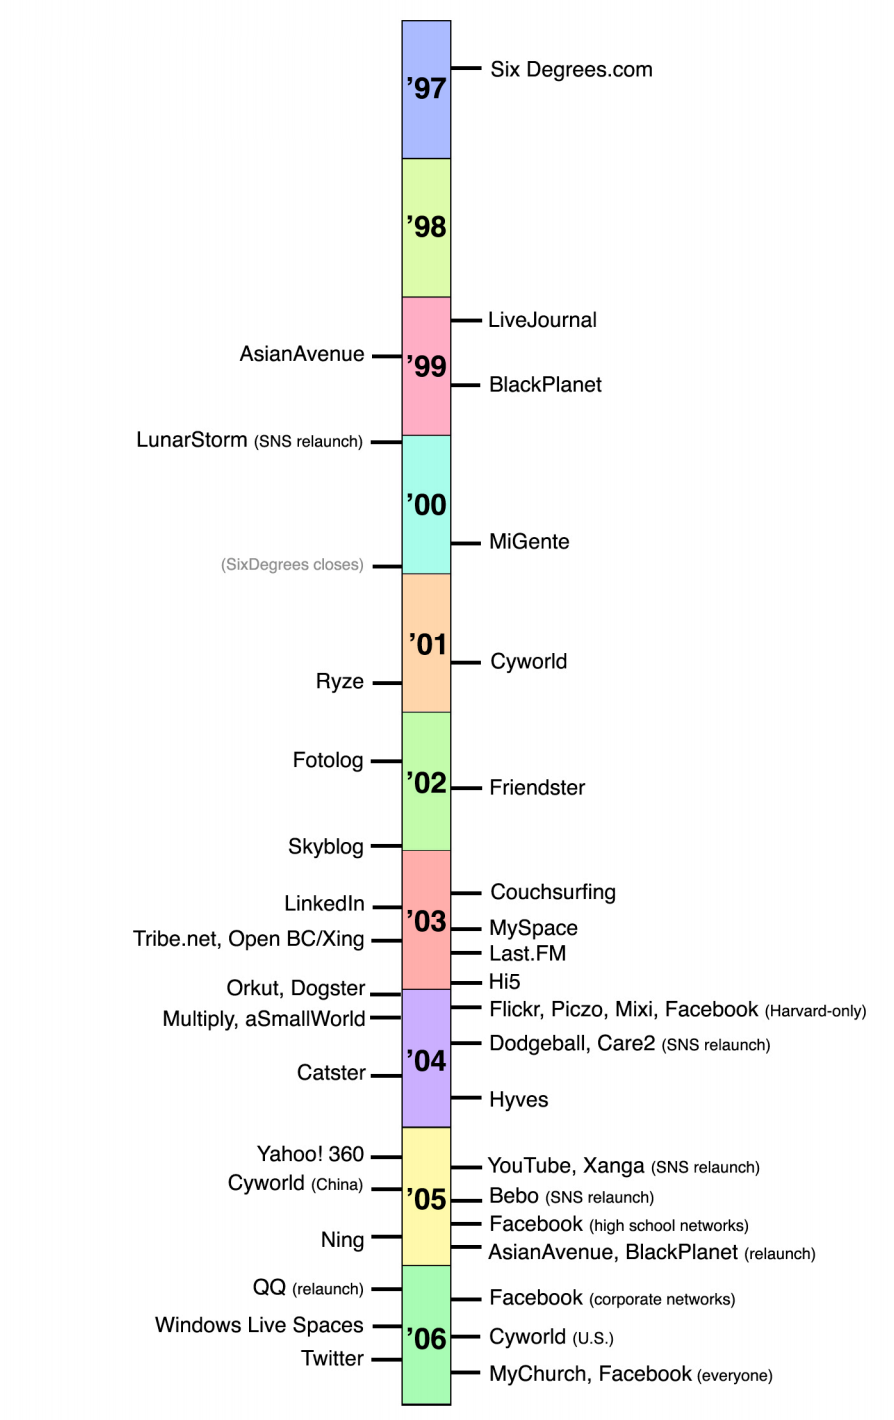
\includegraphics[width=0.7\textwidth]{img/timeline.png}
\end{center}
\caption{\label{img:timeline} Launch dates of major \glspl{osn}.}
\end{figure}

Although the first platform possessing some of the main characteristics that define \glspl{osn} \citep{ellison2007social}, as we can see in Figure \ref{img:timeline}, the first recognizable \gls{osn} launched in 1997 as we can observe in the Figure \ref{img:timeline} \citep{ellison2007social}. \textit{SixDegrees.com} allowed users to create personal
profiles, connect with friends and consult friends of friends lists. The profile feature came from the
online dating sites and online communities, while the surfing through register users in the network
and consulting friends was an existing feature in Classmates.com. \textit{SixDegrees.com} was the first to combine
these features.

\textit{SixDegrees} promoted itself as a tool to help people to connect, but in 2000, it became an
unsustainable business and the service closed. At the time the creators conclude that
\textit{SixDegrees} was a service that was very ahead of its time.

Until 2002 many \glspl{osn} have emerged, but still incapable of projecting themselves at a global scale.
As we can observe in the timeline of Figure \ref{img:timeline} \citep{ellison2007social} from 2002 and 2005 the \textit{big players} came to existence, in these periods, \gls{osn}
such as Friendster, LinkedIn, MySpace, Hi5, Facebook and Youtube were born, shaping the business, cultural
and research landscape.


%% ---------------------------------------------- Portuguese and Online Social Networks
\section{Portuguese People and Online Social Networks}
From Table \ref{table:osns}, we get a good overview on \glspl{osn} usage among modern society. In this section we do a deep exploration of the most adopted \glspl{osn} by portuguese citizens,
and get to compare then with the more global scenario presented in Table \ref{table:osns}, also, other interesting facts will be revealed where appropriate.\\
\indent A recent study, \cite{marktest2016}, revels portuguese relationship with \glspl{osn}. This study, has been made by \textit{Marktest Consulting} since 2011, with the goal of know the notoriety, utilization, opinion
and habits of portuguese concerning social networks. The study information was collected trough online interviews. The sample was built from 819 interviews from individuals with age between
15 and 64 years, living in Portugal and using \glspl{osn} in a daily basis.\\
\indent Some of the most interesting facts revealed in this study, relative to the participants are:
\begin{itemize}
  \item 94\% has a Facebook account and 43\% a Youtube account;
  \item 21\% has abandoned a social network in the past year;
  \item 27\% considers that their dedicated time to social media has increased;
  \item 67\% follows celebrities and 62\% follows brands;
  \item 87\% is used to watch videos in social networks.
\end{itemize}

\indent These are indeed interesting conclusions, but what about the top used \glspl{osn}, \textbf{the most used are
the following (by order): Facebook, Youtube, Google+, LinkedIn, Instagram and Twitter}.\\
\indent Relatively to \cite{marktest2016} past studies, Facebook has maintain
its top position, maintaining a grow tendency that has been standing out in the past years.

\indent Going back to Table \ref{table:osns}, we may now comment the usage of \glspl{osn} by portuguese people comparing it
to the global scenario. As one may notice Facebook still rules users preferences within portuguese.
The other noticeable point is that the \glspl{osn} preferred among portuguese are general propose ones,
but with a slight tendency to content sharing networks (mainly photos).

\indent Concerning to global time related usage statistics, according to \cite{marktest2016}, \textbf{portuguese spend 91 minutes a day with social networks},
68\% considers that this is the ideal time to spent with social media, despite 1 in each 4 saying that in the past year has dedicated even more time to them.
Even if people spent more than one hour and an half in this platforms, the study
concluded that \textbf{67\% of the users that visit \glspl{osn} several times a day only 41\% does daily publications}.

\indent \textbf{The prime time for using \glspl{osn} is between 8pm and 10pm}, being the smartphone the most used device in this time. Also in this short period the
featured \gls{osn} is Facebook, the majority of the interviewed say that is the most credible site, the one that provides better and useful information,
the most interesting and addictive.


%% ---------------------------------------------- Exploring Specific Online Social Networks
%% ---------------------------------------------- Exploring Some OSNs
\section{Exploring Specific Online Social Networks}

In this section we are going to explore in greater detail some of the \glspl{osn} presented
in Table \ref{table:osns}. The selection of the social networks was not aleatory, we are going
to study deeply the \glspl{osn} that gather some important characteristics, that will be of use in
the future when we design the system for analyzing and visualizing social networks. First, the
\gls{osn} must be accessible, this said, one must be capable of extracting information from the platform
in order to analyze it. Second, the \glspl{osn} should preferably be the most diversified as possible, so that we
can draw different types of conclusions deriving from different kind of analysis, for then give proof
of the adaptability of the system to different \glspl{osn}. Considering the previous
comments, these are the following \glspl{osn} that we think that as a group, better represents the intentions
previously mentioned, so we will cover them with more detail (with no particular order):
\begin{itemize}
  \item Facebook;
  \item Instagram;
  \item LinkedIn;
  \item ResearchGate;
  \item Pinterest;
  \item Twitter.
\end{itemize}

%% ---------------------------------------------- Exploring Some OSNs
%% -------------------------------------------------- Facebook
\subsection{Facebook}

Facebook is an \gls{osn}, created by Mark Zuckerberg in 2004, which started out by being an exclusive social network for Harvard students, but came later to spread across
the country and the globe, having today more than one billion users.\\
\indent Before diving into details of Facebook's domain, one must first point out some of its general aspects. Facebook basically allows anyone with a valid email address to create a public and personalized profile,
we say personalized in terms of displayed content or information such as profile photo, name, work, homeland, education etc. .
The next fundamental step is connect with other users, by sending friendship requests to other Facebook users (this are bidirectional relations).
The base entity of the network is the user, but entities such as brands, companies can also be part of the platform, appearing normally
in the form of page, being a page a public place inside the network with marketing or business related purposes (celebrities, public institutions also use pages as form of appearing in Facebook).\\
\indent The next parts of this section will clarify the roles of this entities and their way of interact with each other, also other important concepts will be presented.

\subsubsection*{Domain Model}

\begin{figure}[h!]
  \hspace*{-0.5in}
  %% -- PROPOSTA DE NOVA FORMA DE APRESENTAÇÃO VERTICAL --
  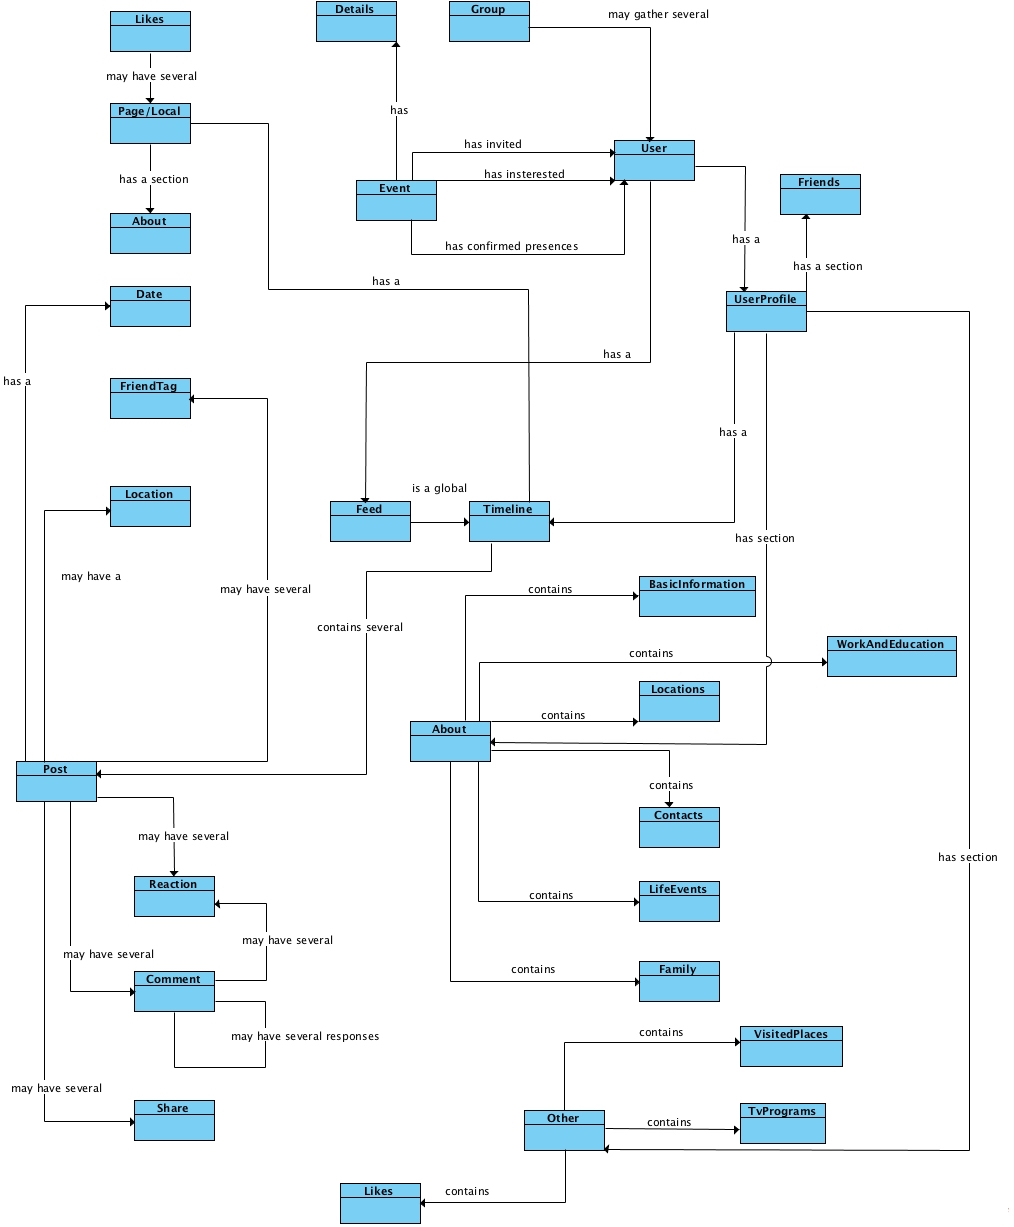
\includegraphics[width=1.10\textwidth]{img/facebook-domain-model.jpg}
\caption{\label{img:fbdomain} Facebook domain model schema.}
\end{figure}

\indent In this section we explore the domain of Facebook represented in Figure \ref{img:fbdomain} in detail, what are the pieces that conceptually build
this platform, and how they relate. The schema in Figure \ref{img:fbdomain} represents a macroscopic perspective among Facebook components and their organization.\\
\indent There are two entities with bold labels in the schema, this are, \textbf{User} and \textbf{Post}, being
\textit{User} the base entity in the network (the node in the network graph basically), and \textit{Post} the most basic unit of content sharing in Facebook.\\
\indent Facebook is interesting in terms of data gathering, because despite offering users' basic information
and to whom that users are related (\textit{Friends} box), it has a collection of other interesting data
such as the family relationships (\textit{Family} box), geographical locations where the user lives, or
visited locations (\textit{Locations} and \textit{VisitedPlaces} boxes respectively), and among other things, user information
may contain the personal interests that were explicitly inputed by the user (\textit{Likes} box).\\
\indent In what concerns to user activity in the platform, the \textit{Timeline}, provides all the user
Posts chronologically ordered, this is where Facebook dynamism takes place, users are constantly
adding content to their timeline, it may be life related events or simply sharing other users posts linking content. The user feed (\textit{Feed} box) represents
a global timeline where the user can consult all the posts on his network (this is by default the user's landing page on the platform).\\
\indent Facebook has, with time, become more then a user profile centralized network, it has invested in expand its horizons, becoming
the place where pages of brands, companies, organizations (media, political, non-profitable etc.), or places (cities, monuments, bars etc.) live (\textit{Page/Local} box).
This entities that are now cohabiting with users in the Facebook ecosystem, take advantage of the platform and its range to get their updates to most people as possible. The profile
for these pages are in many ways different form the user's profile, it also has a timeline, but the about information and other details represent a smaller part of page's profiles,
the most important metric for pages is its number of \textit{likes} (\textit{Likes} box), it represents the number of users in the network that follow the page, it might be users
that simply have a certain relation with the entity or simply want to keep in touch by regularly receiving these entities updates in their Facebook walls
\footnote{Facebook wall an area where users can see the posts of their friends and/or liked pages, in a chronological order}.\\
\indent Other Facebook entities not yet mentioned, are events (\textit{Event} box). These are events inputed in the platform that allow
users to keep updated about relevant events happening mainly in their area. Users can tag the event as \textit{interested in}, showing their friends
the will of participating in some event, or they can simply reject the event. Users also can confirm participation on events
showing their network that they will be present. Events keep three separated counters for users, they count the number of invited users, number of
interested users and number of confirmed users (these relations are expressed as links between the \textit{Event} box and the \textit{User} box).\\
\indent In Facebook is also possible to join groups of users, this groups may be public or private, and they generally are focused on a specific matter,
or gather users from one same institution or organization (e.g. Facebook group of students of the University of Minho).
Having this feature of groups, clustering users by they interests one may say that groups, some way, transform Facebook in a \textit{"multi interest-based \gls{osn}"}.

\subsubsection*{Facebook Graph API}
Facebook has today several software \textit{kits} for developers to interact with the platform in the most diversified and imaginable ways. Facebook developers
offers a range of variated software products that vary from monetization programs, that focus on how to make users profit from Facebook, Analytics to developers who
have their apps embedded in the Facebook platform understand their audience and the performance of their apps, etc. (\cite{fbproducts}).\\
\indent In this master's thesis context, the relevant software that Facebook has available is the Facebook Graph API. This API basically allows developers to collect information
from Facebook such as posts, photos, videos, pages etc. According to \cite{fbgapi}, the common scenarios for using the Graph API
are the following: determine whether two people are friends on Facebook; publishing new status and updates, uploading content (photos, video etc.); sharing links. But in this project what we seek is
build the most biggest and detailed network as possible, with analysis and visualization purposes in mind.\\
\indent For building the network fetching users friends information is crucial, this was possible until Facebook Graph API v2.0 (trough the router \textit{/me/friends}), one could actually retrieve
friends information and build a network from there. From v2.0 on, to achieve what was explained before, one must request a special permission called \textbf{user\_friends}
from each user. The permission \textbf{user\_friends} is no longer included by default in every login. This change breaks down the possibility of gather Facebook information via its Graph API,
this said, we need in the future to look up alternative paths to extract data from Facebook.


%% ---------------------------------------------- Exploring Some OSNs
%% -------------------------------------------------- Instagram
\subsection{Instagram}

\begin{quote}
\textit{"Since the beginning, Kevin has focused on simplicity and inspiring creativity through solving problems with thoughtful
product design. As a result, Instagram has become the home for visual storytelling for everyone from celebrities, newsrooms and
brands, to teens, musicians and anyone with a creative passion."} \cite{instabout}
\end{quote}

Similarly to Facebook we are going to explore Instagram in the same way. Instagram was originally developed by Kevin Systrom and Mike Krieger, and launched in 2010, only
for iPhone devices. Within a year Instagram was able to gather around 10 million of users. Later, in 2012 Facebook acquire Instagram for approximately 1 billion dollars.\\
\indent As already mentioned in Table \ref{table:osns}, Instagram does not belong to the group of general purpose \glspl{osn}, instead, Instagram specially focused on photo
and video sharing, building a global community that shares more than 95 million photos every day.\\
\indent According to \cite{instabout}, since
the very beginning Instagram was a very simplistic platform, being this characteristic reflected on its domain model.

\subsubsection*{Domain Model}

\begin{figure}[h!]
  \hspace*{-1in}
  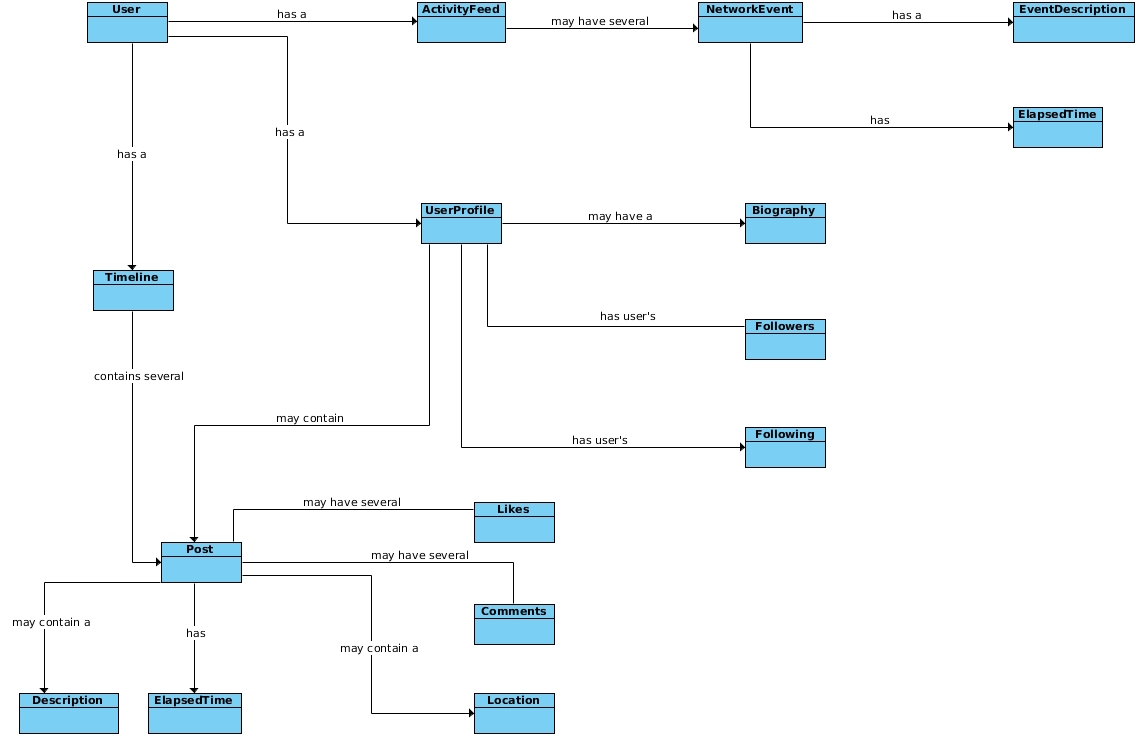
\includegraphics[width=1.28\textwidth]{img/instagram-domain-model.jpg}
\caption{\label{img:instadomain} Instagram domain model schema.}
\end{figure}

Figure \ref{img:instadomain} represents the domain model of Instagram, and as we can observe, simplicity its the essence of this platform, since this diagram is far
more a realistic representation of Instagram than Figure \ref{img:fbdomain} is a representation of Facebook, and this may be why Instagram is so massively adopted by users
on the Internet, because it goes directly to the point, focusing mainly on sharing activity, offering a real easy and simple user experience.\\
\indent Now concerning to the domain model, we can see that a user and its profile (\textit{User} and \textit{UserProfile} boxes) are very simple entities, because
a user's profile is only its biography (\textit{Biography} box), relationships (\textit{Followers} and \textit{Following} boxes) and the user's posts, that despite
being chronologically ordered, do not intend to form any kind of timeline such as Facebook, instead it represents more the concept of a wall with frames hanged on it.\\
\indent In Instagram the landing page, represents a timeline (\textit{Timeline} box) with posts from users we follow. Regarding to posts (\textit{Post} box), one can
comment posts (\textit{Comment} box), but one cannot react or respond to comments (this preserves simplicity even more, for nested comments represent
 a complex part of \gls{osn} such as Facebook), and react to them by the \textit{like} reaction (\textit{Like} box).

\subsection*{Instagram API Platform}
In consequence of a simple domain, Instagram API Platform, provides simple and useful
end points for programmatic publishing, and for network discovering, as far as concerning to this project, the late utility
is more of interest. Instagram allows to get users, their relationships and also the media shared content (posts).\\
\indent Similarly when exploring Facebook Graph API, we now found also very intimidating restrictions for the purpose of this project,
this restrictions include limited rate of 500 API requests per hour, and end point specific limitations that allow only to
perform 30 requests per hour to getting users' relationships data. (\cite{instadev})

%% ---------------------------------------------- Exploring Some OSNs
%% -------------------------------------------------- LinkedIn
\subsection{LinkedIn}

Moving on to the next \gls{osn} we now have LinkedIn. According to \cite{linkabout}, LinkedIn was launched officially on May 5 of 2003, and by the end of
that month, the network had already more than 4500 members. In 13 June of 2016 LinkedIn was acquired by Microsoft in an all-cash transaction valued at \$26.2
billion (\cite{microlink}).\\
\indent LinkedIn is an \gls{osn} that has a very narrow purpose, which is
connecting professionals around the globe to make them more productive and successful.

\subsubsection*{Domain Model}

\begin{figure}[h!]
  \hspace*{-0.5in}
  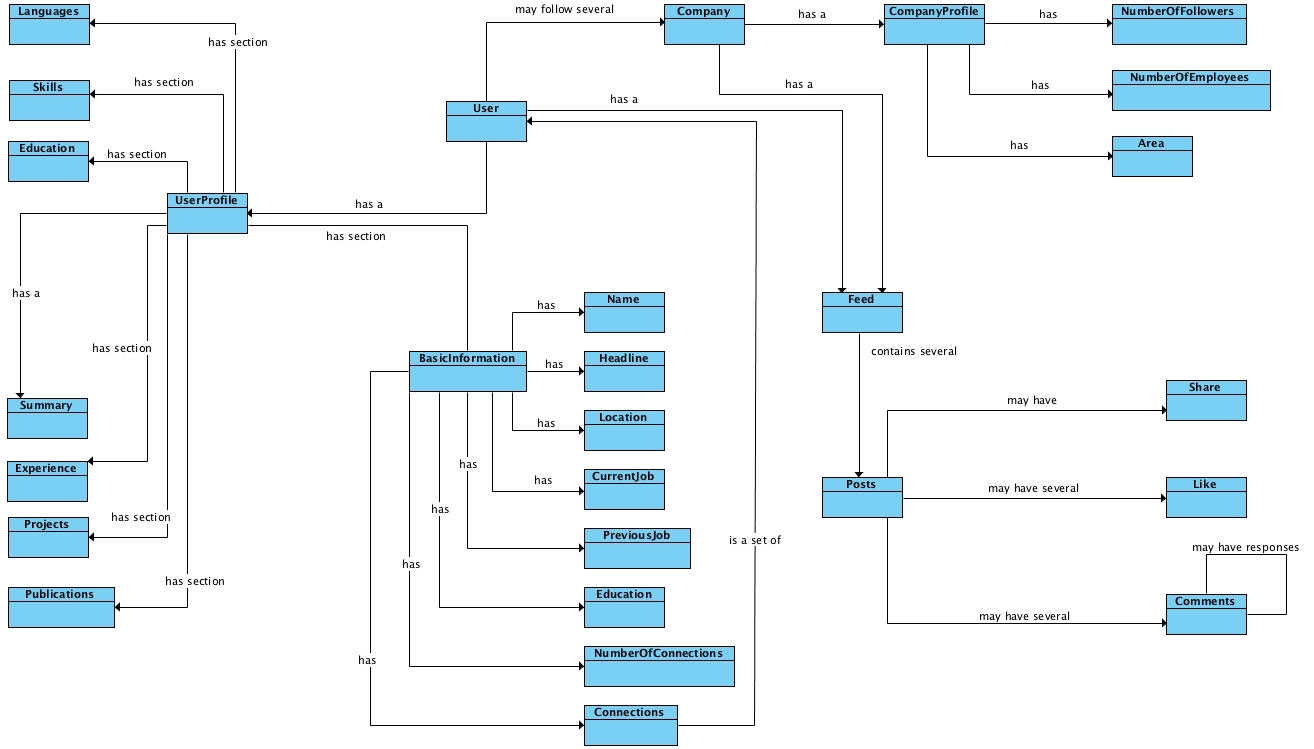
\includegraphics[width=1.10\textwidth]{img/linkedin-domain-model.jpg}
\caption{\label{img:linkdomain} LinkedIn domain model schema.}
\end{figure}

\indent Being a more purpose oriented \gls{osn} and focused on the professional
world, makes LinkedIn platform more complex, even with a simplified representation of the domain model, as we can observe in Figure \ref{img:linkdomain} it is schema
\footnote{\indent In the schema presented on Figure \ref{img:linkdomain}, much of the platform complexity was simplified in order to produce a simple domain, and to narrow
down this analysis to the core components and concepts of LinkedIn.}
far more complex that Instagram, having more or a similar complexity comparing to Facebook.\\
\indent In LinkedIn the user profile (\textit{UserProfile} box) is very rich in terms of what is important for building an individual professional image (profile),
starting by one individual's basic information (\textit{BasicInformation} box) that has information like name, location and current and/or previous jobs. Then
the user profile has several sections with very specific purposes such as professional experience (\textit{Experience} box), languages (\textit{Languages} box) or
education (\textit{Education} box), all this summed up give a very precise perspective of an individual's "professional appearence". At the bottom of the profile
we have along with the professional recommendations and connections, the skills or expertise section (\textit{Skills} box), this is one of the most attractive features
in the LinkedIn platform. Skills in LinkedIn are a tagging system that allow user's to expose their expertise trough their public profile and then receive feedback
on them according to their ability on that specific skill, this is a very important and promising feature for matching user's profiles with
job positions requirements.\\
\indent LinkedIn's main entities are not only users, the industry is massively represented in this network too. Companies may have a company profile
(\textit{Company} and \textit{CompanyProfile} boxes) where they present the company, containing basic information such as number of people following the company
number of employees (giving the idea of the company dimension) and the area where the company fits (pharmaceuticals, technology etc.) (\textit{NumberOfFollowers},
\textit{NumberOfEmployees} and \textit{Area} boxes respectively).\\
\indent Other important concept of LinkedIn is the user feed where the user can chronologically consult a series of posts produced by their connections
or by companies that their follow.

\subsection*{LinkedIn API}
LinkedIn provides a REST API (\cite{linkapi}), but still similarly to the \glspl{osn} we been studying its very limited. In what concerns to data retrieval LinkedIn only allows
the consult of basic profile data, this is the data retried from the LinkedIn interactive REST console:\\

\begin{verbatim}
  {
  "firstName": "Daniel",
  "headline": "Graduate Front-end Developer at Blip.pt",
  "id": "k_yk8W37WH",
  "lastName": "Caldas",
  "siteStandardProfileRequest":  {
    "url": "https://www.linkedin.com/profile/..."
  }
\end{verbatim}

\indent As we can see from the above data sample, we only could fetch some data properties, that would not bring value in terms of network analysis.

%% ---------------------------------------------- Exploring Some OSNs
%% -------------------------------------------------- ResearchGate
\subsection{ResearchGate}

\begin{quote}
\textit{"Founded in 2008 by physicians Dr. Ijad Madisch and Dr. Sören Hofmayer, and computer scientist
Horst Fickenscher, ResearchGate today has more than 11+ million members. We strive to help them make progress happen faster."} \cite{rgate}
\end{quote}

ResearchGate is an \gls{osn} built specifically for scientists, with the goal of easing the task of collaborative research around the globe. ResearchGate
strikes to connect the world of science and make research open to all.
\clearpage

\subsubsection*{Domain Model}

\begin{figure}[h!]
  \hspace*{-1in}
  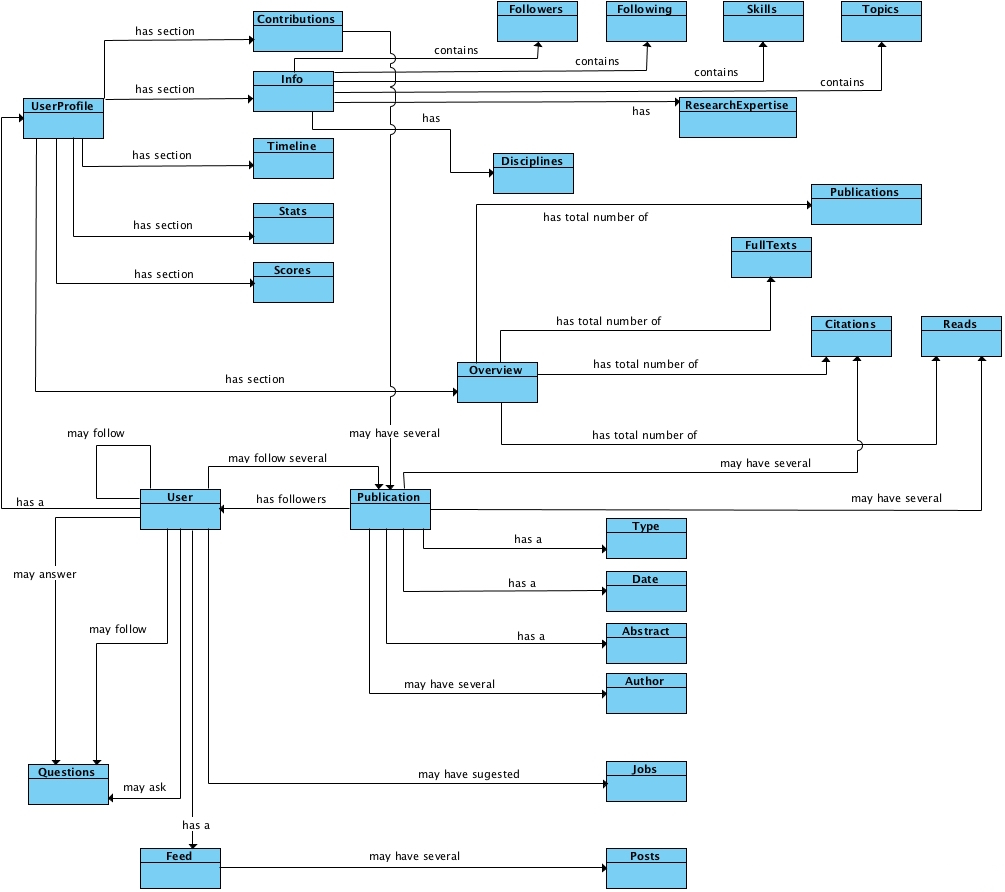
\includegraphics[width=1.28\textwidth]{img/researchgate-domain-model.jpg}
\caption{\label{img:rgatedomain} ResearchGate domain model schema.}
\end{figure}

\subsubsection*{Data Dictionary}
Some terms on the schema presented in Figure \ref{img:rgatedomain} may be quite ambiguous due to the the specificity that they represent. In order to make the schema fully legible and before diving into the domain model analysis, we present first, a small data dictionary detailing the terms one may found more ambiguous:

\begin{itemize}
\item \textbf{Scores} - This term represents a collection of metrics that evaluate the performance of a user based on his contributions and research experience. The user has also associated a global score;
\item \textbf{Topics} - Topics represent the user's scientific areas of interest, ResearchGate uses topics to provide personalized suggestions;
\item \textbf{Disciplines} - Represent more broad areas of the user education, expertise and interest;
\item \textbf{Type} \begin{small}(\textit{Type} box connected with the \textit{Publication} box in Figure \ref{img:rgatedomain})\end{small} - A type classifies a publication, this said, a publication may be an article, a book, a thesis a conference paper etc. .
\end{itemize}

\subsubsection*{Domain Model Analysis}
ResearchGate is a peculiar \gls{osn} that despite having connections between individuals, it has alongside connections between individuals and scientific publications,
making the publication (\textit{Publication} box) a social object, playing the same role that videos play in Youtube for example.\\
\indent Like LinkedIn the user profile (\textit{UserProfile} box), is very detailed and builds up a very clear image of the researches work, positions and areas of interest. The relations
among users are bidirectional, following the followers/following (\textit{Followers} and \textit{Following} box) strategy like other \glspl{osn} such as Instagram or Twitter. Very simillarlly to LinkedIn, a
user's profile has a skills (\textit{Skills} box) section, where skills are expressed in the form of tags, the tag description is far more specific than LinkedIn tags, that may some
times acquire very abstract or high level descriptions (e.g. Technology Information). In ResearchGate tags have are very specific and are
normally related with the user topics (\textit{Topics} box) or disciplines.\\
\indent Publications play along with the user a main role in ResearchGate. Normally publications have associated a type (already explained in the data dictionary section), a date, an abstract and may have one or more authors. The main metrics for Publications rating are the number of reads (\textit{Reads} box) and the number of
citations (\textit{Citations} box) of that publication. The publications may also be followed by users that may have interest on particular publications.\\
\indent Other concept of ResearchGate that raises the collaborative spirit among users, living up to the values that originated the platform, is the questioning system
(\textit{Question} box). Users may ask each other specific questions and have them answered by an expert on a specific scientific area, this opens up the possibility of having
the best experts on a specific matter giving their opinion, thus the possibility of obtaining the \textit{"best possible answer in the globe"}.\\
\indent ResearchGate users' receive open jobs suggestions based on their profile, also user's have a post where they receive activity notifications of the people
or publications that they are following.

\subsubsection*{API}
Today ResearchGate does not provide any API for accessing its data or for any kind of interaction with the platform.

%% ---------------------------------------------- Exploring Some OSNs
%% -------------------------------------------------- Pinterest
\subsection{Pinterest}
According to \cite{pintabout}, Pinterest \textbf{is the world's catalog of ideas}. Created by Ben Silbermann, Paul Sciarra and Evan Sharp and launched in 2010, Pinterest is a simple but yet very original \gls{osn}, instead of aiming for connecting people like Facebook or LinkedIn, it aims for inspire people trough new ideas.

\subsubsection*{Domain Model}

\begin{figure}[h!]
  \hspace*{-1in}
  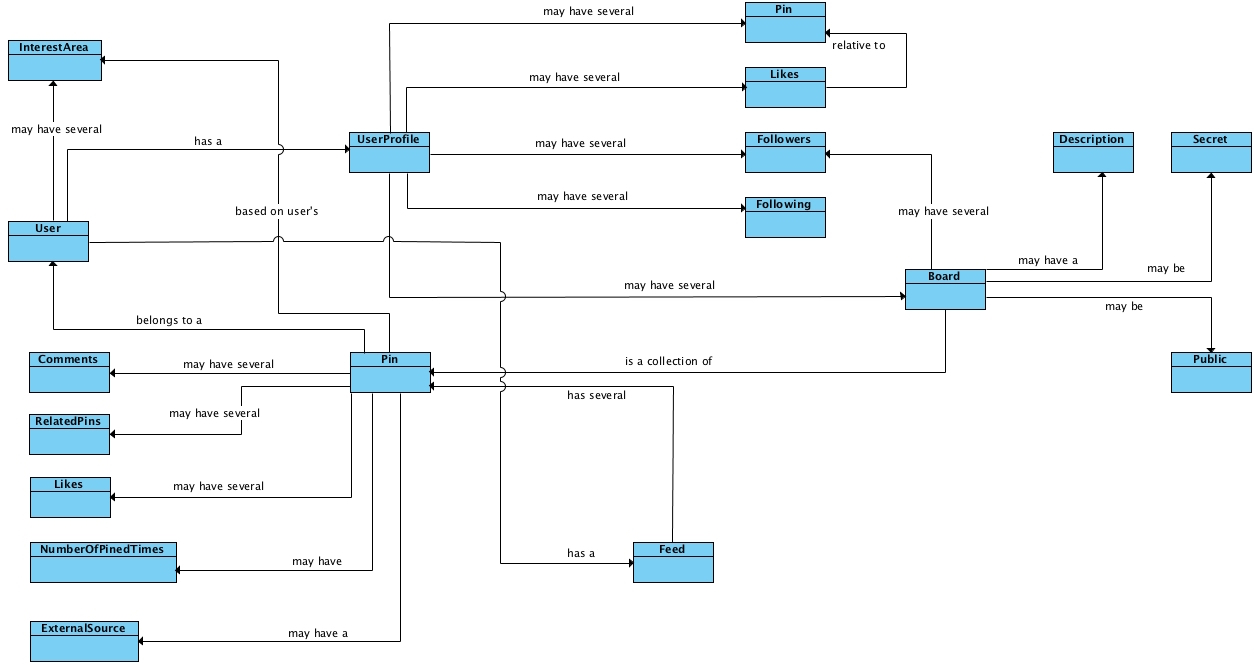
\includegraphics[width=1.20\textwidth]{img/pinterest-domain-model.jpg}
\caption{\label{img:pintdomain} Pinterest domain model schema.}
\end{figure}

\subsubsection*{Data Dictionary}
As one may notice from Figure \ref{img:pintdomain}, Pinterest introduces very particular concepts that may lack explanation, that is why we present first a small data dictionay before going trough the analysis, as we did with ResearchGate on a previous section:

\begin{itemize}
\item \textbf{Pin} - A Pin is the basic unit of Pinterest, it represents an idea of some user, presented in some context (the board context), and it is presented to us with a picture;
\item \textbf{Board} - As the name suggests, a board is a collection of pins. Boards are created from users to other users, and normally present pins within some context (e.g. travels, technology, food etc.). In Pinterest boards may be followed by other users;
\item \textbf{NumberOfPinedTimes} - This entity is not entirely a Pinterest entity, instead it represents a relevant metric introduced to measure pins popularity, and it refers to the act of saving pins. Pins that are presented to the users may be saved (or \textit{"pinned"}), and the number of times that users have saved a particular pin is expressed in Figure \ref{img:pintdomain} by the box \textit{NumberOfPinnedTimes};
\end{itemize}

\subsubsection*{Domain Model Analysis}
Pinterest introduces new concepts forming a very original \gls{osn}, because it's very different from others that we analyzed previously. Just as we seen in ResearchGate, where the domain model is build around a social object (the scientific publication), with Pinterest we have a similar scenario, where the concept of the platform is built around a different social object the Pin (\textit{Pin} box), which also as a grouped perspective introduced by a group or collection of pins that are the boards (\textit{Board} pin). Pinterest is basically a set of pins aggregated in boards that are explored in the platform accordingly to the user's interests.\\
\indent Simmilarly to other networks (e.g. Instagram) Pinterest also has direct unidirectional connections between users that adopt the concept of \textit{"follow/following"} (\textit{Followers} and \textit{Following} boxes). As user's can follow publications in ResearchGate, Pinterest users may follow boards, being then notified if some pin is added to that specific board.\\
\indent In what concerns to Pins, they may be commented by users (\textit{Comments} box), they also may be targeted by likes as posts in Facebook (\textit{Likes} box). A particular point concerning to Pins is that they can have a explicit external reference, for instance, if some image is extracted by some other web site or from other \gls{osn} they can be explicitly referenced, and that same reference appears at the top of the pin along with its title (\textit{ExternalSource} box).\\
\indent Pinterest was the traditional concept of feed, but in this case, the feed represents a completely different concept compared to other \gls{osn}. First the content of the feed (pins) is not related with users we follow on the network, is instead related is our personal interests (\textit{InterestArea} box) and second, they are not presented according to a chronological order, and visually they do not follow the standards of typical timeline/feed design, instead the different pins displayed on some user's feed, form some kind of board or catalog, like the ones people use to hang in walls and pin post-its on it.

\subsubsection*{Pinterest API}
According to \cite{pintdev}, Pinterest provides a REST API for developers interact with the platform. The data restrictions follow Facebook politics, where the application that integrates Pinterest API can only fetch data for authenticated users. Pinterest provides endpoints to interact with users, boards and pins. Concerning to the requests limitation, Pinterest offers a 60 minute sliding window where 1000 requests can be made by unique user token.

%% ---------------------------------------------- Exploring Some OSNs
%% -------------------------------------------------- Twitter
\subsection{Twitter}
One \glspl{osn} that frequently is bring to discussion for being more of a \textit{"news content generator"} is Twitter. Twitter is another of must most used \gls{osn}
listed in Table \ref{table:osns}, is basically a social networking microblogging service that allows their users to broadcast short posts (short because they're maximum size cannot exceed the 140 characters) called tweets.
Twitter was created in March 2006 by Jack Dorsey, Noah Glass, Biz Stone, and Evan Williams, gaining fast worldwide popularity, Twitter has today more then 300 Million users according to Table \ref{table:osns}.\\

\indent Unlike many other social networks that have private or semi-public profiles with restrict policies concerning to exterior access to information within the network (examples of this kind of \glspl{osn} may be LinkedIn or Facebook),
Twitter default settings are public, making tweets spread more effectively across all social media, this particularity makes Twitter one of the most \textit{"barrier-free}" \glspl{osn}. Of course that despite unregistered people may read tweets
they cannot interact with them as Twitter users by linking, comment or \textit{"retweet"}\footnote{The act of retweet consists and share some existent tweet originated by another user.} them.

\clearpage

\subsubsection*{Domain Model}

\begin{figure}[h!]
  \hspace*{-0.4in}
  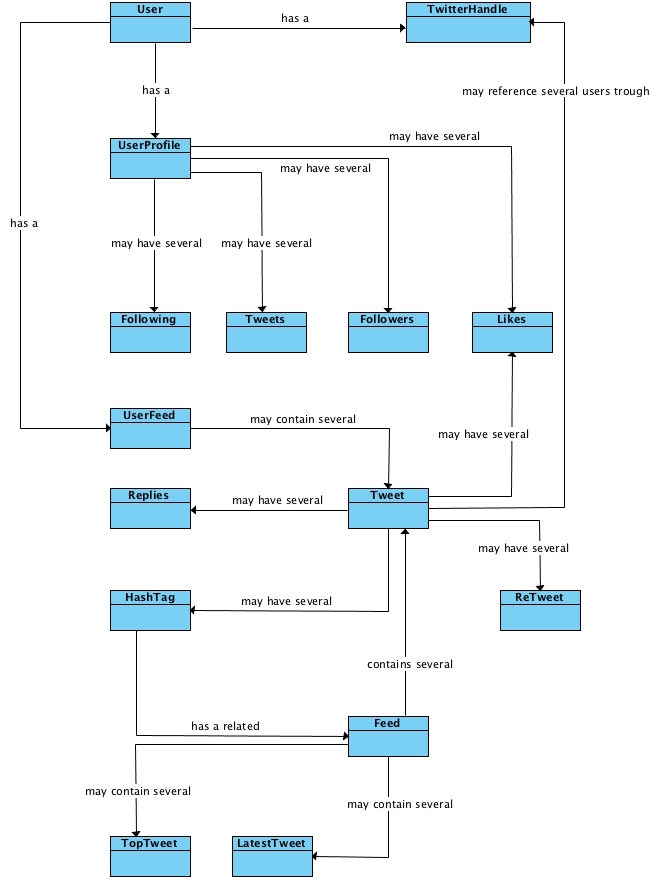
\includegraphics[width=0.9\textwidth]{img/twitter-domain-model.jpg}
\caption{\label{img:twitter} Twitter domain model schema.}
\end{figure}

\subsubsection*{Domain Model Analysis}
In Figure \ref{img:twitter} on may observe a very concise representation of the Twitter domain. Despite being a very minimalist \gls{osn}
concerning to data properties and relationship complexity, Twitter has some very semantically strong features that brand the platform, being those
features used among other well known \glspl{osn} such as Facebook. We are referring specifically the hashtag ((\textit{HashTag} box) and the (\textit{TwitterHandle} box),
but let us first introduce some of the more basic features.\\

\indent As usual in these kind of platforms, Twitter's users posses a user profile
(\textit{UserProfile} box) that as attached to it some properties and user metrics such as number of followers, number of tweets, number of
other users the user is following, and number of likes the user has obtained across all his or her tweets (\textit{Followers}, \textit{Tweets}, \textit{Following}, \textit{Likes} boxes respectively).\\

\indent The tweet is the basic unit of Twitter, is trough tweets that information flows in Twitter. Also tweets may have several comments, and they may
be \textit{retweeted}. Now back to hashtags and twitter handles. Hashtags is in some way how these chaos of unstructured tweets gain some semantic
value, in order to a group tweets according to a specific matter. Hashtags may in many cases be misleading, because users
start to adopt hashtag to express sentiments or simply describing a tweet pushing back to the already mentioned unstructured chaos.
Twitter handles are the same as tags in Facebook they serve as a mean to mark a specific twitter user, a twitter handle may be used in a comment or
in a tweet leading directly to the respective user's twitter profile.

\subsubsection*{Twitter API}
Similarly to other \glspl{osn}, twitter provides a REST API to fetch users data such as profile data, tweets or user's followers. Restrictions are felt
again this API is very limited providing a 15 minutes window for making http requests.

\subsubsection*{Other data sources}
\label{sec:otherdatasources}
As more and more of \gls{osn} appear to be closing doors to data availability even when for research purposes one may
want to search for alternative data sources to feed the system that we intend to build along this project. Projects as
KONECT (\cite{kunegis2013konect}) provide large data sets of networks collected online so that researchers may
perform all types of operations and experiments on that data. This kind of alternatives are very valuable in terms of network
analysis even for real time data analysis systems that may in a more immature phase of the project benefit from this data sets.

\begin{quote}
\textit{"KONECT (the Koblenz Network Collection) is a project to collect large network datasets of all
types in order to perform research in network science and related fields, collected by the Institute
of Web Science and Technologies at the University of Koblenz–Landau."} \cite{kunegis2013konect}
\end{quote}

%% ---------------------------------------------- Exploring Some OSNs
%% -------------------------------------------------- Summary
\subsection{Summary}
In this section we have explored with some detail six of the \glspl{osn} listed in the Table \ref{table:osns}. In this analysis we followed a similar approach for analyzing each \gls{osn}, adding only an additional step for the more domain specific \glspl{osn}, that were ResearchGate and Pinterest, which was building a small data dictionary in order to ease the interpretation of the domain model schema.\\
\indent From the analysis we may draw some generic conclusions concerning the domain of each \gls{osn}. Despite the differences and specifics of each platform, all them sum up to the basic primitive concepts of social networks, that are \textbf{actors} and \textbf{relational ties} between them, which form \textbf{subgroups} originating \textbf{groups} that build the network. This being the high level conclusion for our analysis, there are other patterns that emerge when analyzing different \glspl{osn} like the \textbf{user profile} that is a key element characteristic of this platforms and \textbf{feeds} (or \textbf{timelines}) that represent a standardized way of communicating events within a \gls{osn}.


%% ---------------------------------------------- How Online Social Networks Have Changed The World
\section{How Online Social Networks Have Changed The World}

Social media have clearly shifted the way we communicate and we perceived the world, simply putting it, nowadays with social media one can say that social media is responsible for \textit{"everyone talking to everyone about everything all of the time"}.\\
\indent In fact, 62\% of the entire adult population in on social media \citep{demogsmu}. As an example of events that were clearly influenced by social media, we have the presidential campaign of Barack Obama in the United States, started in 2007 and ended in 2009, Barack Obama had as his campaign technological adviser Chris Hughes, co-funder of Facebook, who played a crucial role in the campaign through online social media. The outcome of the election of 2009 could have been very different without the online social media.\\
\indent Very interesting reflections are made on how social media impacts the world \citep{6wayschange}, and the six major drawn conclusions are the following: \textbf{across industries, social media is going from a \textit{“nice to have”} to an essential component of any business strategy}; \textbf{social media platforms may be the banks of the future}, as an example we have the bank customer profiling through social media in order to get a loan; \textbf{social media is shaking up healthcare and public health}, because information is spreaded \textit{at the speed of light} through social media, this means less struggle to achieve public health  and well-being awareness; \textbf{social media is changing how we govern and are governed}, with \glspl{osn} public participation has grown and everyone can participate in their opinion making people voices louder, bringing more credibility to the democratically system implemented by many governments across the planet; \textbf{social media is helping us better respond to disasters}, as the health public awareness improved through social media information propagation speed, so did improved the response of governments and institutions to disasters such as natural disasters, in countries that may have not the services or infrastructure to respond to some catastrophes, making social media and crucial component to raise awareness across the globe, that have impact in help mobility, or fund raising for supports the damages made by certain disaster; \textbf{social media is helping us tackle some of the world’s biggest challenges, from human rights violations to climate change}.\\
\indent If we look particularly to the most globally used \gls{osn} there are in \textit{"seven ways Facebook has changed the world"} \citep{relrevfacebook}, we are going to point and comment out some of the most relevant. \textbf{Facebook has changed the definition of friend}, if back there having a dozen of friends was already a very large number of relationships, with Facebook the new limit was raised up to the hundreds or thousands of friends, the concept was given a completely new meaning, since we don't need to know a person face to face so that one becomes friend with the other, one simply needs to click the \textit{"add friend"} button, and it does not matter if it is one's neighbor or some other person on the another side of the planet; \textbf{We care less about privacy}, \textit{"if you are not paying for it, you are the product"}, means that we are not paying for using Facebook or any other \glspl{osn}, this said we must retain that these online platform profits from our information and from our interactions, but even being the majority of the users aware of this situation, that doesn't seems to bother anyone; \textbf{Facebook has created millions of jobs – but not in its own offices}, for example the marketing industry suffer a revolution since the raise of the social media, there are jobs for people to manage business and brands profiles on \glspl{osn} it's also a new way to approach customers, as we have seen previously with banks; \textbf{Facebook has been the tool to organize revolutions}, protests and awareness campaigns are raised inside facebook, this is related to the political influence and awareness capacity that we previously have pointed out in this same section.\\
\indent Now switching to the negative aspects of not only Facebook but \glspl{osn} and social media in general. Very strong campaigns were raised against social media, for instance, \href{http://www.imdb.com/title/tt3333168/}{\textit{"The Anti-Social Network"}} a short film depicting a life of an adult which as become obsessed with social networking at the point he starts to break boundaries between his real life and his virtual one. Strategically or ironically these campaigns use social media to spread the word.\\
\indent We have seen that social media had a great deal of impact in society, what about our bodies?  There are numeral studies on this matter, focusing on finding the true negative impacts of \glspl{osn} on
our personal health. Scans to brains of people how excessively use social media, point out that there is a clear degradation of white matter similar to people who are addicted to substances such as drugs or alcohol \citep{lin2012abnormal}, in the regions that control emotional processing, attention and decision making, because social media gives immediate reward (instant feedback) with very small effort, this causes the brain rewire itself make us to desire these stimulations \citep{berridge1998role}. Another common situation among \glspl{osn} users is the idea of multitasking, the felling that one is able to being productive in some task while browsing on social media. Users who heavily use social media are more susceptible to interference from irrelevant environmental stimuli \citep{ophir2009cognitive}, leading these users to perform worse on a test of task-switching ability, because they were not able to filter out interferences.




	% CHAPTER 4 - Social Network Analysis -------------------------
	\chapter{Social Network Analysis}
	%% ---------------------------------------------- Chapter Introduction

% Social network analysis is the application of network theory to the modeling and analysis of social systems.
% it combine both tools for analyzing social relations and theory for explaining the structures that emerge from the social interactions.
%
% Of course the idea of studying societies as networks is not a new one but with the rise in computation and the
% emergence of a mass of new data sources, social network analysis is beginning to be applied to all type and
% scales of social systems from, international politics to local communities and everything in between.
%
% Traditionally when studying societies we think of them as composed of various types of individuals and organizations,
% we then proceed to analysis the properties to these social entities such as their age, occupation or population, and them ascribe quantitative value to them.
%
% This allows social science to use the formal mathematical language of statistical analyst to compare the values of
%  these properties and create categories such as low in come house holds or generation x, we then search for quasi
%  cause and effect relations that govern these values.
%
% This component-based analysis is a powerful method for describing social systems. Unfortunately though is fails to
% capture the most important feature of social reality that is the relations between individuals, statistical analysis
% present a picture of individuals and groups isolates from the nexus of social relations that given them context.
%
% Thus we can only get so far by studying the individual because when individuals interact and organize, the results
% can be greater than the simple sum of its parts, it is the relations between individuals that create the emergent
% property of social institutions and thus to understand these institutions we need to understand the networks of social relations that constitute them.
%
% Ever since the emergence of human beans we have been building \glspl{sn}, we live our lives embed in networks
% of relations, the shape of these structures and where we lie in them all effect our identity and perception of the world.
%
% A social network is a system made up of a set of social actors such as individuals or organizations and a set of
% ties between these actors that might be relations of friendship, work colleagues or family. Social network science
% then analyze empirical data and develops theories to explaining the patterns observed in these networks
%
% In so doing we can begin to ask questions about the degree of connectivity within a network, its over all structure,
% how fast something will diffuse and propagate through it or the Influence of a given node within the network. lets take some examples of this
%
% Social network analysis has been used to study the structure of influence within corporations, where traditionally
% we see organization of this kind as hierarchies, by modeling the actual flow of information and communication as a
% network we get a very different picture, where seemingly irrelevant employees within the hierarchy can in fact have significant influence within the network.
%
% Researcher also study innovation as a process of diffusion of new ideas across networks, where the oval structure
% to the network, its degree of connectivity, centralization or decentralization are a defining feature in the way
% that innovation spreads or fails to spread.
%
% Network dynamics, that is how networks evolve overtime is another important area of research, for example within Law
% enforcement agencies social network analysis is used to study the change in structure of terrorists groups to identify
% changing relations through which they are created, strengthened and dissolved?
%
% Social network analysis has also been used to study patterns of segregation and clustering within international politics
% and culture, by mapping out the beliefs and values of countries and cultures as networks we can identify where opinions and beliefs overlap or conflict.
%
% Social network analysis is a powerful new method we now have that allows us to convert often large and dense data sets
% into engaging visualization, that can quickly and effectively communicate the underlining dynamics within the system.
%
% By combine new discoveries in the mathematics of network theory, with new data sources and our sociological understanding,
% social network analysis is offering huge potential for a deeper, richer and more accurate understanding, of the complex social systems that make up our world.


% RATIONALE
% As the Web rapidly evolves, Web users are evolving with it. In an era of social
% connectedness, people are becoming increasingly enthusiastic about interacting,
% sharing, and collaborating through social networks, online communities, blogs,
% Wikis, and other online collaborative media. In recent years, this collective
% intelligence has spread to many different areas, with particular focus on fields
% related to everyday life such as commerce, tourism, education, and health,
% causing the size of the Web to expand exponentially.
%
% The distillation of knowledge from such a big amount of unstructured
% information, however, is an extremely difficult task, as the contents of today’s
% Web are perfectly suitable for human consumption, but remain hardly accessible
% to machines. The opportunity to capture the opinions of the general public about
% social events, political movements, company strategies, marketing campaigns, and
% product preferences has raised growing interest both within the scientific
% community, leading to many exciting open challenges, as well as in the business
% world, due to the remarkable benefits to be had from marketing and financial
% market prediction.
%
% Existing approaches to big social data analysis mainly rely on parts of text in
% which sentiment is explicitly expressed, e.g., through polarity terms or affect
% words (and their co-occurrence frequencies). However, opinions and sentiments
% are often conveyed implicitly through latent semantics, which make purely
% syntactical approaches ineffective. In this light, this Special Issue focuses on
% the introduction, presentation, and discussion of novel techniques that further
% develop and apply affective reasoning tools and techniques for big social data
% analysis. A key motivation for this Special Issue, in particular, is to explore
% the adoption of novel affective reasoning frameworks and cognitive learning
% systems to go beyond a mere word-level analysis of natural language text and
% provide novel concept-level tools and techniques that allow a more efficient
% passage from (unstructured) natural language to (structured) machine-processable
% affective data, in potentially any domain.

\acrfull{sna} is the study of how people are connected to each other, basically it studies a set of relations among a set of entities,
these entities may be individuals, organizations, or even countries.\\\\
\indent The common analysis procedure consists in mapping the network and then creating metrics to
characterize the network. Then one tries to figure what is the structure of the network and why does
it have that structure. \glspl{sna} is also about looking at the individuals inside the network and where are those individuals located.

%% ---------------------------------------------- Fundamental Concepts for Network Analysis
\section{Fundamental Concepts for Network Analysis}

According to \cite{wasserman1994social}, the concepts listed below are of key importance to understand \glspl{sna}.

\begin{itemize}
    \item \emph{Actor} - \gls{sna} is concerned with understanding the linkages among social entities and the implications of these linkages, these social entities are described as actors. Actors are  discrete individual, corporate, or collective social units.
    \item \emph{Relational Tie} - Actors are linked to one another trough \textit{social ties}. The type of ties may be extensive, and it describes the nature of the connection. Some example of ties:
        \begin{itemize}
            \item \textbf{Evaluation} of one person by another;
            \item \textbf{Transference} of resources (business transactions);
            \item \textbf{Association} (to social event or cause);
            \item \textbf{Behavioural} interactions (communicating);
            \item \textbf{Moving} between places or statuses (migration, social or physical mobility);
            \item Others may be: physical connection (roads, rivers), formal relations (authority), biological relationship.
        \end{itemize}
    \item \emph{Dyad} - The most basic relationship that can be established is a dyad, a connection between two actors.
    \item \emph{Triad} - A relation established between three actors. Many studies included breaking \glspl{sn} down to small groups (triads), this allowed a more clear conclusion about the transitivity of the connections.
    \item \emph{Subgroup} - It defines any subset of actors in a \gls{sn} (conceptually, subgroups come after dyads and triads).
    \item \emph{Group} - A finite set of actors who for conceptual, theoretical or empirical reasons are treated as a finite set of individuals in which network measurements are made.
    \item \emph{Relation} - A collection of ties of a specific kind among members of a group is called a \textbf{relation} (e.g. a connection in \textit{LinkedIn} is a relation while evaluating our connections of sending them messages are ties).
    \item \emph{\gls{sn}} - With the definitions of actor, group and relation, a \gls{sn} consists of a finite set or sets of actors and the relation or relations defined on them. The presence of relation information is critical and defining feature of a \gls{sn}.
\end{itemize}

%% ---------------------------------------------- Graphs Theory
\section{Graphs Theory}
Graphs are typically the base of representation of social structures. This mathematical approach maps with  extreme convenience social networks. Nodes are individuals, and edges are relationships. Despite looking a quite simple approach, there is a very strong theoretical background that is of basilar importance for interpreting social networks.

%% ---------------------------------------------- Statistics
%% \section{Statistics}
%% ...

%% ---------------------------------------------- Network Analysis
\section{Network Analysis}
In this section we intent to explore the scientific concepts behind network analysis, always trying to map them to reality, so only the core
and applicable concepts will be explored in this section, namely:

\begin{itemize}
\item \textbf{\textit{Power Laws}} - Power laws or power law distribution, represent in general a dependency relationship between two quantities. In \glspl{sn}, power law distribution describes a particular trend in the evolution of the number of relationships of individuals within a network;
\item \textbf{\textit{Random Graphs}} - Radom graphs are a way of generating one of the possible graph within the universe of possibilities of a given number of nodes and a given number edges. This graphs are used to map predictions to real networks;
\item \textbf{\textit{Centrality Measures}} - Centrality measures aim to answer the following question \textit{\textbf{Which vertices are important?}}. In a \glspl{sn}, an actor centrality measures the actor's interactions with other individuals;
\item \textbf{\textit{Link Analysis}} - Link analysis is a well known term form web search engines, popularized by the Page Rank algorithm. In \glspl{sn}, link analysis measures individuals connections, such as identifying strongly connected nodes, absorbing nodes or even cycles inside networks;
\item \textbf{\textit{Community Detection}} - Community detection is related to clustering in social networks. Normally when analyzing \glspl{sn} we aim for detecting communities (groups) that express similar ideas in matters such as politics, music or philosophy. Community detection is a far more abstract concept than geographical clustering, despite we often found in \glspl{osn} such as Facebook, that the two concepts are tightly coupled;
\item \textbf{\textit{Spread of Information}} - Spread of information consists in a set of metrics that classify the propagation of the information within a network. Considering a Facebook post by a newspaper, it would come in hand to know, where was the starting point of that post, how many individuals it reaches, in which sub-networks the information was propagated, what were the entry points of for that sub-networks, how fast the information got to the individuals, these are some of the concerns relating to spread of information;
\item \textbf{\textit{Social Learning}} - Social learning consists in the change of behavior or beliefs based on direct observation of other individuals. Considering again a Facebook post by some random individual A, and consider an individual B that shares ('\textit{re-posts}') the individual's A post. If one detects a pattern in this kind of interaction, one may say that individual B is learning from individual A (imitating, mirroring).
\end{itemize}

%% ---------------------------------------------- Small World Problem
\section{Small World Problem}
This principle of \textit{small-world phenomenon} is based on the idea that all human beings are connected by \textbf{short chains of acquaintances}. The pioneer of this work was Stanley Milgram.

\subsection*{Six Degrees of Separation}
The concept of six degrees of separation is an extension of the small world problem. In the sequence of what we state before, the six degrees of separation materialize the previous concept in six interconnections for some individual to reach any other one. Six degrees of separation gained a particularly strong relevance, when a play was written in the 90's portraying the concept.

\section{Network Visualization}
Network visualization may be considered as a science by itself. In this section we will explore some relevant techniques for graph representation and visualization, we will look in particular, into \cite{beck2014state}, where a good overview is made upon graph representation approaches. We will also in a later phase of this project mentioned the graph representation technologies explored and used in this project.


%% ---------------------------------------------- Social Network Analysis Software
\section{Social Network Analysis Software}
\label{sec:snas}

\begin{quote}
\textit{"(...) more sophisticated graphics capabilities should make exploratory studies using visual displays of networks more fruitful. One should be able to display actor attributes and nodal or subgroup properties (such as expansiveness, centrality, or clique membership) along with the graph. (...)"} \citep{wasserman1994social}
\end{quote}

Next we present some relevant software tools on \glspl{sna}.

\subsection{Structure}

\indent \indent The program Structure \citep{structure-software} is a free software package mainly used to investigate population structure. Its uses include inferring the presence of distinct populations, assigning individuals to populations, studying hybrid zones, identifying migrants and admixed individuals, and estimating population frequencies in situations where many individuals are migrants or admixed.

\subsection{Gephi}

\indent \indent Gephi \citep{bastian2009gephi} is a tool for keen data analysts and scientists who want to explore and understand graphs. Like Photoshop™ but for graph data, the user interacts with the representation, manipulates the structures, shapes and colors to reveal hidden patterns. The goal is to help data analysts to make hypothesis, intuitively discover patterns, isolate structure singularities or faults during data sourcing. It is a complementary tool to traditional statistics, as visual thinking with interactive interfaces is now recognized to facilitate reasoning. This is a software for Exploratory Data Analysis, a paradigm that appeared in the Visual Analytics field of research.

\subsection{UCINET}

\indent \indent UCINET 6 \citep{ucinet-software} for Windows is a software package for the analysis of social network data. It was developed by Lin Freeman, Martin Everett and Steve Borgatti. It comes with the \textbf{NetDraw} \citep{borgatti2002netdraw} network visualization tool.

\subsection{SocNetV}

\indent \indent Social Network Visualizer \citep{socnetv} is a cross-platform, user-friendly application for the analysis and visualization of Social Networks in the form of mathematical graphs, where vertices depict actors/agents and edges represent their relations.

With SocNetV you can construct social networks with a few clicks on a virtual canvas or load field data from various social network file formats such as GraphML, GraphViz, Adjacency, Pajek, UCINET, etc.

Furthermore, you can create random networks using various random models.

\subsection{networkx}
\indent \indent networkx \citep{hagberg2013networkx} is a Python language software package for the creation, manipulation, and study of the structure, dynamics, and functions of complex networks. networkx relevant features are listed below:
\begin{itemize}
    \item Python language data structures for graphs, digraphs, and multigraphs;
    \item Many standard graph algorithms;
    \item Network structure and analysis measures;
    \item Generators for classic graphs, random graphs, and synthetic networks;
    \item Nodes can be "anything" (e.g. text, images, XML records);
    \item Edges can hold arbitrary data (e.g. weights, time-series).
\end{itemize}

\subsection{Vizster}

\textbf{Vizster} \citep{heer2005vizster} is a tool for Visualizing online social networks, a visualization system for playful end-user exploration and navigation of large-scale online social networks.

\subsection{Project Palantir (Facebook)}

\textbf{Project Palantir} \citep{project-palantir} \footnote{This project is not at the level of \glspl{sna} specificity of the previous tools, still we consider worth mention it.} is an impressive tool that displays the rate of interactions on Facebook across the globe. This was a result of an intern annual event that happens in Facebook where all the employees are invited to participate and to build creative prototypes in the context of the company.


\section{Real World Applications}
Here we will present some of the real world applications of social networks analyzes with special attention for developed projects with a similar focus to this master's dissertation, and other tools of \glspl{osn} that cross many fields of studies. Two examples of projects with similar focus to this master's dissertation are:

\begin{itemize}
    \item \textit{\textbf{Vizster}} (\cite{heer2005vizster}) - Visualizing online social networks. A visualization system for playful end-user exploration and navigation of large-scale online social networks;
    \item \textit{\textbf{Project Palantir}} (\cite{project-palantir}) - This is an impressive tool that displays the rate of interactions on Facebook across the globe.
\end{itemize}


	% CHAPTER 5 - System Architecture Proposal -------------------------
	\chapter{System Architecture Proposal}
	Before diving into the architectural details of the system, we first present a state of the art summary, that concisely describes what is the positioning of this project in light of the previous explored \glspl{sna} tools that we presented in chapter 4, and also considering the \glspl{osn} that we study in chapter 3.\\
\indent Specifically regarding the \glspl{sna} tools, we will comment some of them, some of their useful features and overall comments to what may lack on this tools that this project may target, in order to differentiate and not only \textit{''reinvent the wheel''}.

\section{Simplicity}
Aside of \textbf{Vizster} \citep{heer2005vizster}, the majority of the previously presented tools such as Gephi \citep{bastian2009gephi} or Social Network Visualizer \citep{socnetv}, are very complex tools with very heavy interfaces, that have a big learning and are meant for users that have particular advanced knowledge in \glspl{sn} and \glspl{sna}. The tool to be developed could also serve for less expert users, providing a set of core basic functionalities (e.g only allow users to load and visualize they're networks), and then, allow the user to build complexity from there enabling and disabling other features.

\section{Accessibility}
All the software that we presented above exists in the form of desktop applications. This applications need to be downloaded, and installed in a compatible machines (sometimes with dependencies on other software that is not installed by default). Nowadays almost every application is web based, this allows users to access them every where through a browser, making web apps a solution that is Operating System and device agnostic. This said, building a web based social networks analysis tool could be a way of tackle the accessibility of such tools.\\
\indent A web based application, it's good for sake of accessibility but in another hand it is a performance culprit when it comes to performance. This is a decision to take into account, but always having in mind that tackling performance it's not the main goal this master's thesis, also, the mentioned tools are mature projects that are highly performant and are capable of rendering huge networks.

\section{\acrfull{osn} integration}
Social Network Visualizer \citep{socnetv}, allows to \textit{scrap} web sites to build networks, but for this feature relies only on links to build the network (it blindly scraps recursively some url to build the network). By allowing the user to analyze networks that are directly reporting they're social network status would be a differentiation factor from the other tools, and would certainly be a more meaningful and valuable analysis for the end user.

\section{Drawing Accurate Conclusions}
As we state before when talking about simplicity, the mentioned \glspl{sna} tools provide generic metrics on networks such as network density or actor centrality. The values outputted from this tools are the result of running generic formulas and algorithms against some networks, so its very common for current \glspl{sna} researchers to be worried about the size of the network, being their focus on \textbf{quantitive analysis}.\\
\indent In a hypothetical analysis scenario where some researcher has a network with a few thousand nodes, \textbf{what is the meaning of his assumptions when analyzing the network}? Since this is a pure quantitive analysis the numbers will seem reasonable for the given network, but this will not allow him to extract contextual conclusions, because in this case analyzing data from Facebook or analyzing data from LinkedIn will sound just like the same, it would all comes down to the network. A better approach for drawing conclusions would be to have a mixture between \textbf{quantitive analysis} and \textbf{quality analysis}, the tool could do some content and context analysis, to help the end user on achieving more meaningful conclusions, rather than just some numerical metrics.

\section{System positioning and tools comparison}
In this section we will make a high level comparison between the software tools presented in chapter 4. In Table \ref{table:toolscompare} we can observe the tools classification based on some predefined metrics that show the positioning of the proposed system, these metrics are:

\begin{itemize}
    \item \textbf{Availability (Desktop or Web)} - Whether the tool available through a desktop application or a web application;
    \item \textbf{Complexity (Low, Moderate, High)} - Whether the tool has very complex features that require expertise to be used, also we may consider the learning curve for using the tool with efficiency;
    \item \textbf{Performance (Low, Medium , High)} - Whether the tool is performant, if it computes metrics with velocity and if it renders dense graphs without struggle;
    \item \textbf{Network Edition (Yes, No)} - Whether the tool allows network editing, such feature allows adding nodes and edges to existing network or event creating new networks from scratch;
    \item \textbf{\glspl{osn} Integration (Yes, No)} - Whether the tool is able to integrate data analysis of \glspl{osn}.
    \item \textbf{Contextual Analysis (Yes, No)} - By contextual analysis we do not mean that the user will not be aware of the network context, our contextual analysis has a strong meaning, it represents the capacity that the system demonstrates (or not) to be aware of the context of the network and providing metrics with a specific meaning.
\end{itemize}

\begin{table}[H]
\hspace*{-0.9in}
\renewcommand{\tabcolsep}{2pt}
\begin{tabular}{ |c|c|c|c|c|c|c|c|  }
\hline
\textbf{Tool} & \textbf{Availability} & \textbf{Complexity} & \textbf{Performance} & \textbf{Network Edition} & \textbf{\glspl{osn} Integration} & \textbf{Contextual Analysis}\\
\hline
\textbf{Structure} & Desktop & Moderate & Medium & Yes & No & No\\
\hline
\textbf{Gephi} & Desktop & Moderate & Good & Yes & No & No\\
\hline
\textbf{UCINET} & Desktop & High & Very Good & Yes & No & No\\
\hline
\textbf{SocNetV} & Desktop & Low & Medium & Yes & No\footnotemark{}\addtocounter{footnote}{-1} & No\\
\hline
\textbf{\begin{tabular}{@{}c@{}}Our system\\projections\end{tabular}} & Web & Low & Low & No & Yes & Yes\\
\hline
\end{tabular}
\caption{\label{table:toolscompare} Software tools comparison and our system positioning.}
\end{table}

As we can observe in Table \ref{table:toolscompare} our system has essentially three differential factors, that are: web availability; \glspl{osn} integration; contextual analysis; being the trade off for such gains the system performance. When describing our system compared to the other tools we want to be able to have a web tool that has a complexity level similar to SocNetV\footnote{\label{socnetv-footnote}SocNetV has a feature that allows the user to launch a \textit{web spider} that navigates through web sites building a network representative of the links between the sites, but the \textit{spider} is not content aware, it blindly builds a network without context.}.

\section{System Architecture}

Now, after building up our aiming for this project, we now present a more concrete image of the overall system. In Figure \ref{img:architectureprop} we present an abstract system architecture.

\begin{figure}[h!]
\begin{center}
  \hspace*{-0.8in}
  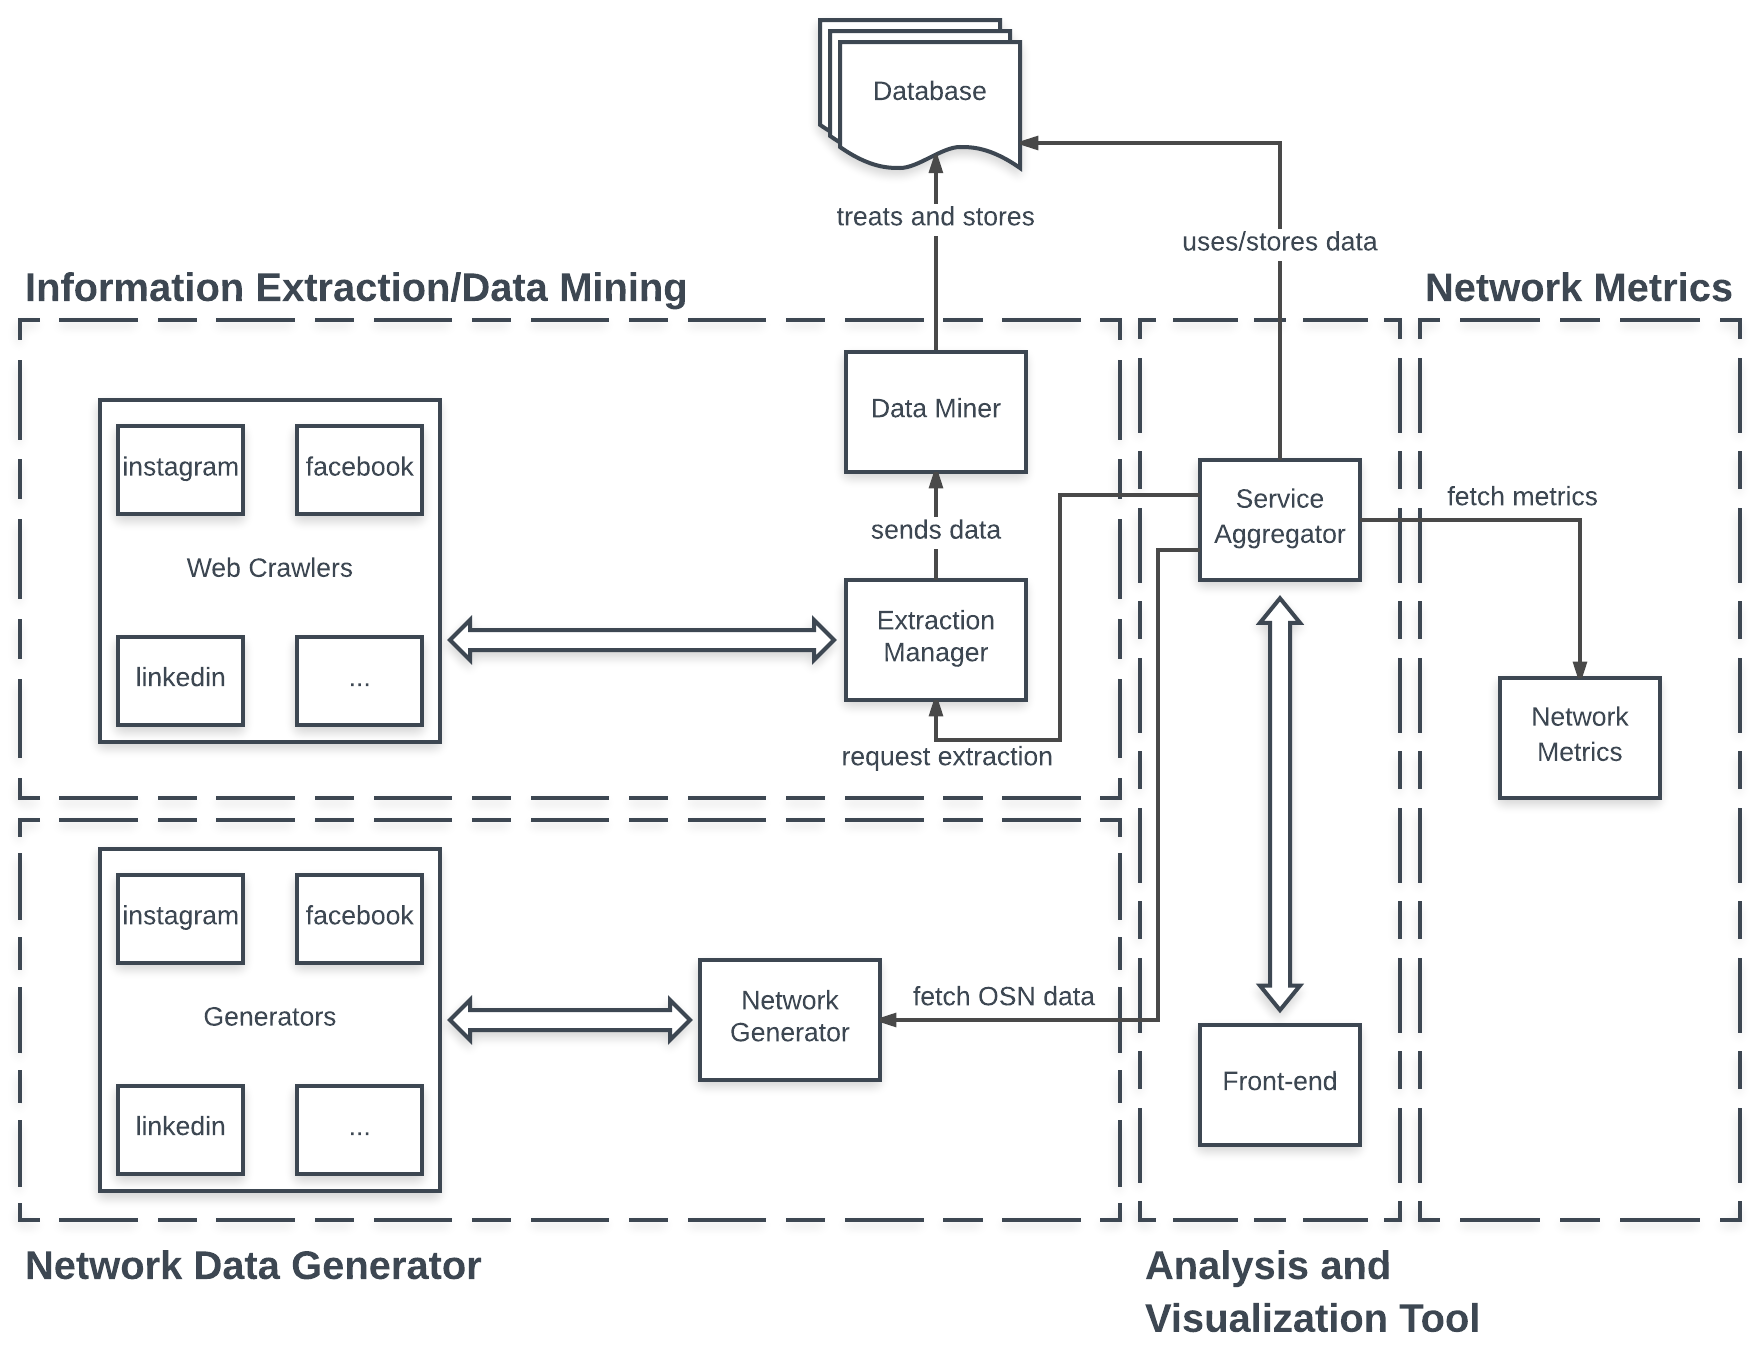
\includegraphics[width=1.2\textwidth]{img/architecture_v3.png}
\end{center}
\caption{\label{img:architectureprop} System architecture proposal.}
\end{figure}

\subsection{General overview}
As the interaction of the software components may be clear from the diagram, the role of each module is not clear by simple
diagram observation, an underlying explanation of each component is needed in order to understand the system.\\
\indent We will follow a \textit{top down} approach for explaining the system architecture. First let us be clear about the two
main and distinct parts of the system:
\begin{itemize}
    \item \textbf{\textit{Information extraction and data mining}} - All the other components are built for extracting information
    from existent databases, or from \glspl{osn} (through the \textbf{Web Crawler}) and store information being information properly treated before stored;
    \item \textbf{\textit{Network Data Generator}} - For sake of a ease of development process, and also to assure a fallback strategy upon information extraction failure, we create a network generator module that basically generates data models confined to the data schemas that we previously presented for Facebook and LinkedIn;
    \item \textbf{\textit{Network metrics}} - This module acts as a isolated component that is dedicated to perform calculations and algorithms on stored networks. It will feed metrics as requests by other components;
    \item \textbf{\textit{Analysis and Application/Visualization}} - The tool that directly interacts with the end user is composed by a \textbf{Service Aggregator} that fetches data from a database, requests extractions to the application back-end and runs calculations and algorithms on top of stored networks as the user requests by interacting with a \textbf{Front-end} that provides the visualization and interaction features.
\end{itemize}

\subsection{Detailed Components Description}
The components presented in Figure \ref{img:architectureprop} more detailed explanation, next we look more carefully into each on of the components.
\begin{itemize}
    \item \textbf{\textit{\acrfull{osn}}} - This are the object of study, the source of information that the systems will process and analyze;
    \item \textbf{\textit{Web Crawler}} - The \textbf{Web Crawler} consists in a set of modules for crawling each one of the \glspl{osn} (\textit{fb-extraction} and other modules);
    \item \textbf{\textit{Extraction Manager}} - This module consists in a wrapper for extracting information from social networks, and allows extraction orchestration spreading extraction processes along multiple hosts, so that we can mitigate the slowness of web crawlers and extraction process in general;
    \item \textbf{\textit{Data Miner}} - The data mining process assures that we store a well defined data schema that describes in the more simplified way the state of the networks;
    \item \textbf{\textit{Database}} - The database is where we store our data. It is not represented by the \textit{classical cilindro} because it resembles relational databases, and the possibility of using non relational databases such as document databases, grows strongly within the project, and the reason is the unstructured data that we will be storing into our database. We also plan on feeding some data through already existing databases, instead of crawling data from \gls{osn}. This databases may be provided from projects that we already mentioned in this document  (\hyperref[sec:otherdatasources]{Section 3.3.6}), such as \citep{kunegis2013konect}. This data would be accessed through the \textbf{Data Miner}, or a new module could be constructed exclusively to feed this data to our database;
    \item \textbf{\textit{Generator}} - a generator is a simple module that creates contextualized sets of data in order to fed our front end with the expected data that would come from the extraction module;
    \item \textbf{\textit{Network metrics}} - These module fetches data directly from the database in order to perform network operations that may be heavy. Isolating this component will allow logic separation from the service aggregator and will allow a separated infrastructure deploy, so that we may have dedicated computer resources on network metrics calculations;
    \item \textbf{\textit{Service Aggregator}} - Ideally this component application will read the already normalized information from the database, run \glspl{sna} calculations and algorithms against the stored networks, and request data to the back-end (the Information extraction and data mining super component). The Service aggregator is also responsible for communicating with network measures component in order to fetch metrics about a given network as the user requests to access it;
    \item \textbf{\textit{Front-end}} - The front-end will render the networks to the user, and will allow the user to interact with the network; these interactions will be defined in the requirements specifications.
\end{itemize}


	% CHAPTER 6 - System Requirements -------------------------
	\chapter{System Requirements}
	In this Chapter we will specify with detail the system requirements and particular features to be implemented. The requirements
will be divided in two major sections.\\
\indent First we will describe what tasks the Back-end of the system should perform in order to provide
all the data and tools for supporting the system Front-end. Then with the end user in mind we will define the tool requirements from
the user point of view. For aggregator that is part of the Front-end no requirements will be specified since this component will only bridge
requests from the Front-end and the Back-end or will eventually fetch data directly from the database.\\

\section{Social Networks Prioritization}
Before diving into the requirements we first will review our \glspl{osn} preferences regarding information extraction and the
interest we have in analyzing this specific networks.\\
\indent First we want to analyze \textbf{Facebook} because it is the more general purpose network, the more popular and the more used
thus allowing us to derive more interesting conclusions since the resultant graphs will be more realistic having a more concrete social structure
representation. Second we want to analyze \textbf{LinkedIn} because it is also widely used and the only one that specifically
focus on professional worldwide networking, generating different kinds of graphs and understand how companies and professionals
are interacting online. Analyzing LinkedIn may also introduce an interesting analysis that is merging information from Facebook and
analyzing friendship networks within professional networks.\\
\indent Having two networks embedded in the system proves that we can analyze social networks in general since we have more
than one and with different purposes, but since the system is designed to simply accommodate new networks simply adding
a new extraction module should the major part of the work to integrate a new \glspl{osn}, this said we could eventually
also implement some extra modules to the remaining \glspl{osn} listed in Chapter 3.

%% ---------------------------------------------- Back-end
\section{Back-end}

As seen is Figure \ref{img:architectureprop}, our Back-end is essentially composed by two parts: \textbf{web crawlers/extraction modules}; \textbf{extraction manager} and the \textbf{data miner}. We will write the requirements for each one of the components. We will not prioritize these requirements (as we will do in the \hyperref[sec:frontend]{next section for the Front-end} requirements) because \textbf{all listed requirements are essential for the overall system usefulness}.

\subsection{Web crawlers}

Each web crawler (or extraction module) must fulfill common requirements that are listed below \footnote{These requirements are agnostic to the \glspl{osn} context}:

\begin{enumerate}
    \item Web crawlers should be able to login with a user account (an \textit{entry point});
    \item Web crawlers should be able to navigate through the pages of a given \gls{osn};
    \item Web crawlers must be capable of performing "human" interactions such as click and scroll;
    \item Web crawlers should be able to output a predefined (agreed and formally defined in the next section) data schema, covering eventual
    exceptions due to privacy limitations;
    \item Web crawlers must be able to perform user extraction with second order depth, from the user entry point perspective (this means that we want to extract user's friends and friends of friends information);
    \item Extraction modules should provide a global extraction method where extraction parameters can be passed from the outside reducing or amplifying the scope of extraction as specified from the outside (e.g. under given circumstances we may only need to extract the friends' list or the basic information like name, city and birth date);
    \item Extraction modules must be available to the data miner through a web \gls{api} in order to allow remote and distributed extraction. The web \gls{api} must wrap all the different supported \glspl{osn} being each one accessible through a different path within the same web \gls{api}. The extraction web \gls{api} required specifications are presented next:
    \begin{itemize}
        \item \textbf{GET /api/v1/extraction/\{osn\}} - should return a confirmation message signalizing that \gls{api} is up and ready for receiving requests;
        \item \textbf{GET /api/v1/extraction/\{osn\}/\{user\_id\}} - should perform full extraction of the user with the \textit{user\_id} in the \textit{osn} ;
        \item \textbf{POST /api/v1/extraction/\{osn\}/\{user\_id\}} - should receive a set of options, that parameterize the extraction and reduce the scope of the extraction for a given \textit{user\_id} within some \textit{osn}.
        \item \textbf{POST /api/v1/extraction/\{osn\}/} - same as the previous but instead of performing extraction for a given \textit{user\_id}, performs it to a set of \textit{user\_ids} performing multiple extractions;
        \item In \gls{api} version 1 \textbf{osn} must be one of the following: \textbf{facebook}, \textbf{linkedin};
        \item \textbf{user\_id} is a string that uniquely represents the user within a specific \gls{osn}.
    \end{itemize}
\end{enumerate}

\subsection{Extraction Manager}

Below are the extraction manager requirements \footnote{Again, these requirements are agnostic to the \glspl{osn} context}:

\begin{enumerate}
    \item Orchestration of extraction processes scattered across various hosts: one should be able to define a list of hosts and the number of extraction processes that each host should handle;
    \item Chunk an entry point (that is a set of user identifiers within the \glspl{osn}) in order to delegate different users to different hosts;
    \item Call the extraction endpoints according to the \glspl{osn} from where we need to extract data.
\end{enumerate}

\subsubsection{Extraction pipeline}

\begin{figure}[h!]
\begin{center}
  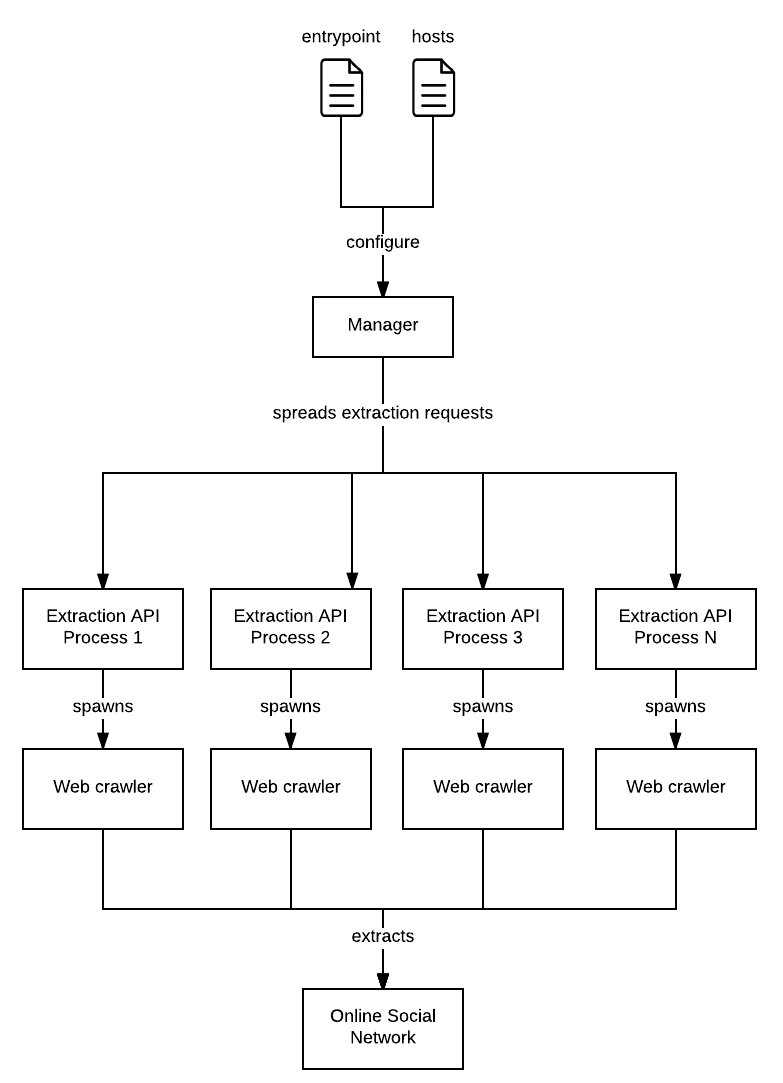
\includegraphics[width=0.7\textwidth]{img/ext-pipeline.png}
\end{center}
\caption{\label{img:extpipeline} Extraction pipeline diagram.}
\end{figure}

Being listed above the requirements for each component we will now draw the specification of what is the expected workflow for data extraction, in Figure \ref{img:extpipeline} we design a pipeline that tries to reflect, with maximum detail, the listed requirements. The diagram does not cover the data mining process that is responsible for normalizing data and store it. This diagram is exclusively focused on how we pretend that data extraction is achieved in order to mitigate the slowness of web crawlers.\\
\indent As we can see from Figure \ref{img:extpipeline} we aim to follow a very straight forward process in order to extract information. First we provide an entry point for a given \glspl{osn} (the user the web crawlers will use to log in into the social platform), and a hosts file that describes the resources available for extractions, this is intended to be simply a list of hosts (ip addresses) that have the extraction web \gls{api} running and awaiting for extraction requests.\\
\indent Next each extraction \gls{api} instance is responsible for handling a session of some web crawler instance and waits for it to return data so the extraction API instance  can give it back to the extraction manager.

\clearpage

\subsection{Data miner}
\label{sec:dataminer}

The data miner simply assures some data treatment before storing it on the database, that said there is a very narrow requirements list for this component:

\begin{enumerate}
\item Receive extraction data and normalize the fields that may need some treatment giving as result a normalized data structure;
\item Store normalized data in the database;
\item Assure that the data schemas (these are presented in the next section) are well defined.
\end{enumerate}

\subsubsection{Data schemas}

Defining data schemas in earlier stages of system specifications will allow us to develop the Front-end and the Back-end simultaneously, we must for that consider that the only source of true when it comes to data structures is a well agreed contract between both parts. The data miner will assure that the next presented schemas are stored in the database. For convenience reasons we will describe the data structures with a JSON like notation.

\subsubsection{Facebook data structure}
\begin{verbatim}
{
    "uid": {string},
    "livesIn": {
        "id": {string},
        "description": {string}
    },
    "life_events": {
        {string}: [{string}]
    },
    "birthDate": {string},
    "likes": {
        {string}: {string}
    },
    "friends": [{string}],
    "relationships": {
        "civil_status": {
            "id": {string},
            "description": {string}
        },
        "family_members": [
            { "id": {string}, "relationship": {string} }
        ]
    },
    "from": {
        "id": {string},
        "description": {string}
    },
    "name": {string},,
    "gender": {string},
    "age": {number},
    "posts": [
        {
            "timestamp": {string},
            "description": {string},
            "author": {string},
            "reactions": {
                "likes": {number},
                "love": {number},
                "laugh": {number},
                "sad": {number},
                "angry": {number},
                "surprise": {number}
            }
        }
    ]
}
\end{verbatim}

\subsubsection{LinkedIn data structure}
\begin{verbatim}
{
    "uid": {string},
    "name": {string},
    "headline": {string},
    "from": {string},
    "summary": {string},
    "experience": [
        {
            "company": {string},
            "position": {string},
            "duration": {
                "count": {number},
                "unit": {string},
                "from": {string},
                "to": {string}"
            }
        }
    ],
    "education": [
        {
            "institution": {string},
            "course": {string},
            "startYear": {number},
            "endYear": {number}
        }
    ],
    "skills": {
        {string}: {number}
    },
    "languages": {
        {string}: {string}
    },
    "projects": [
        {
            "name": {string},
            "date": {string},
            "description": {string}
        }
    ],
    "groups": [
        {string}
    ],
    "following": [
        {string}
    ],
    "connections": [
        {string}
    ]
}
\end{verbatim}

\subsection{Network metrics}
\label{subsec:networkmetrics}

In this section we will list the requirements for the module that is responsible for calculating metrics upon our stored networks. This component must
provide a web \gls{api} in order to access all the algorithms and metrics calculations that the service offers.

\begin{enumerate}
    \item The \gls{api} must be able to calculate strongly and weakly connected components;
    \item The \gls{api} must be able to calculate the clustering coefficient for a given network;
    \item The \gls{api} must be able to calculate the average neighbor degree;
    \item The \gls{api} must be able to calculate centrality measures, these include:
    \begin{enumerate}
        \item Degree centrality;
        \item Closeness centrality;
        \item Betweenness centrality;
        \item Eigenvector centrality;
    \end{enumerate}
    \item The \gls{api} must be able to compute node importance through the page rank algorithm.
\end{enumerate}


%% ---------------------------------------------- Front-end
% This should be one of my major arguments when talking on static rendering and network perception through time!
% https://en.wikiquote.org/wiki/Edsger_W._Dijkstra - Related cool stuff
% Our intellectual powers are rather geared to master static relations and that our powers to visualize processes evolving in time are relatively poorly developed. For that reason we should do (as wise programmers aware of our limitations) our utmost to shorten the conceptual gap between the static program and the dynamic process, to make the correspondence between the program (spread out in text space) and the process (spread out in time) as trivial as possible.
% \textbf{\textit{"You can think of networks as vast fabrics of humanity, and we all occupy particular spots within the network. Nicholas Christakis}} \url{https://www.youtube.com/watch?v=wadBvDPeE4E&t=1133s}"

\section{Front-end}
\label{sec:frontend}

The Front-end is actually where the majority of the requirements work is, since we need to go into detail of how the user will interact with the tool, we must decide how those interactions will be drawn so that the tool can actually be what it was meant to, also bear in mind that these represent the tool requirements, what the user actually will able to see.

\subsection{Requirements Prioritization}
For simplifying the prioritization process we will use the \textbf{MoSCoW} method \citep{clegg1994case} that is a simple method to define what requirements are more important for the system overall functionality, allowing us to focus on the very essential requirements for getting a functional product \footnote{In this section we will tend to use some terms often find in requirements engineering that may seem a bit off topic, still we find that this is the more objective way for describing our prioritization method}.\\
\indent Next we present the MoSCoW method as it is defined in requirements engineering.

\begin{itemize}
    \item \textit{\textbf{M}ust} have requirements are critical requirements that are part of the identity of the product, they must by all means be implemented.
    \item \textit{\textbf{S}hould} have requirements are definitely important, but they are not critic to the product definition, and they are not time critic as well having the possibility of being included in later stages of the implementation. Some times these requirements may have another ways of satisfying the customer.
    \item \textit{\textbf{C}ould} have requirements are indeed the \textit{nice to have} requirements, being often left outside of the first deliver, but seen as very valuable to the future of the product in later stages of the product time line.
    \item \textit{\textbf{W}on't} have requirements that are agreed to not be included in the first deliver of a project, this does not exclude the possibility of including them in later stages of the project. \textit{Won't} requirements may be seen as future work.
\end{itemize}

The requirements will be listed by groups (sections) that aggregate common requirements or features. Each requirement will have a classification according the MoSCoW method.

\subsection{Network configuration and construction}

In this group of requirements we present a set of requirements that represent the operations that allow the users to get their network built.

\begin{enumerate}
    \item \textbf{[MUST]} The user must be able to generate a network for available \glspl{osn};
    \item \textbf{[MUST]} The user must be able to choose the number of nodes for a certain network and which metrics he wants to compute for that network;
    \item \textbf{[MUST]} The user must be able to register available \glspl{osn} accounts in the system;
    \item \textbf{[MUST]} The user must be able to order the build of its network for a given \gls{osn};
    \item \textbf{[MUST]} The system must give feedback on the extraction status;
    \item \textbf{[COULD]} The user must be able to \textit{blacklist} from the network nodes with a minimum or maximum number of connections;
    \item \textbf{[COULD]} The system must clearly warn the user about the impacts that extracting some kind of data (e.g. extracting complete list of user's likes on Facebook) could have on extraction time and consequently on render network time (these could be expressed via label warnings in the user's interface);
    \item \textbf{[COULD]} The user must be able to \textit{blacklist} nodes specific from being extracted and consequently rendered on the user's graph;
    \item \textbf{[WON'T]} After the first extraction all the extracted nodes must be marked as extracted, being the user able to extract the missing properties for some given nodes.
\end{enumerate}
% Extraction granularity
% \begin{enumerate}
%     \item \textbf{Facebook}:
%     \begin{enumerate}
%         \item \textit{Relationships} - If this flag is checked, relationships will be included;
%         \item \textit{Personal} details - If this flag is checked, personal details will be included;
%         \item \textit{Life events} - If this flag is checked, life events will be included;
%         \item \textit{Posts} - If this flag is checked, most recent posts will be included.
%     \end{enumerate}
%     \item \textbf{LinkedIn}:
%     \begin{enumerate}
%         \item \textit{Experience} - If this flag is checked, experience will be included;
%         \item \textit{Education} - If this flag is checked, education will be included;
%         \item \textit{Skills} - If this flag is checked, skills will be included;
%         \item \textit{Languages} - If this flag is checked, languages will be included;
%         \item \textit{Projects} - If this flag is checked, projects will be included;
%         \item \textit{Groups} - If this flag is checked, groups will be included;
%         \item \textit{Connections} - If this flag is checked, connections will be included.
%         \item \textit{following} - If this flag is checked, following will be included.
%     \end{enumerate}
% \end{enumerate}

\subsection{General interactions and display}

These requirements express general behavior of the tool, and some display features.

\begin{enumerate}
    \item \textbf{[MUST]} The system must be able to render a graph using the information provided by the aggregation service;
    \item \textbf{[MUST]} The system should be able to automatically identify communities by painting nodes belonging to the same community by the same color and providing
    information about the community such as \textit{"People that studied at School/University X"} or \textit{"People that live in city Y"};
    \item \textbf{[MUST]} The user must be able to drag and drop the graph to any place on the graph render area;
    \item \textbf{[MUST]} The user must be able to zoom in and zoom out the network so he is able to explore specific parts with more detail;
    \item \textbf{[MUST]} The user must be able to select two nodes at the same time in order to compare them all values should be displayed side by side in order to provide a practical way to compare two individuals at any level;
    \item \textbf{[SHOULD]} The user should be able to choose activate animations despite these have been deactivated by the system for sake of graph interactions performance ;
    \item \textbf{[SHOULD]} The system should be able to automatically deactivate heavy graph animations if a large graph is being rendered;
    \item \textbf{[COULD]} The user should be able to enable and disable \textit{fisheye distortion} alike effect; % https://bost.ocks.org/mike/fisheye/
    \item \textbf{[WON'T]} The user must be able to perform a \textit{hive plot} \footnote{hive plots define a linear layout for nodes, grouping nodes by type and arranging them along radial axes based on some property of data} of his network;
    \item \textbf{[WON'T]} Double clicking on a empty zone should perform a smooth zooming effect on that area. %https://bl.ocks.org/mbostock/3828981
\end{enumerate}

\subsection{Node interactions}

Here we describe interactions at the node level.

\begin{enumerate}
    \item \textbf{[MUST]} Along side the node a label with the node name or id should be displayed;
    \item \textbf{[MUST]} The user must be able to activate highlight functionality for more interactive node consulting. This functionality will highlight the node and his first degree connections, clarifying relations within very dense clusters; % http://link-prediction.herokuapp.com/network
    \item \textbf{[MUST]} When the user clicks a node a side panel must be opened, this panel should display the following:
    \begin{enumerate}
        \item Should contain all node user's available information;
        \item Should allow the user to perform calculations on that specific node;
        \item Should allow user to request extraction of more information on that node (e.g. if the list of user's likes wasn't extracted this option should be available);
        \item Should offer the user all the metrics already mentioned the previous \hyperref[subsec:networkmetrics]{network metrics section 6.2.4}.
    \end{enumerate}
    \item \textbf{[MUST]} The user must be able to drag and drop the node to some place else in the screen and the node should be fixed in that place (being the rest of the graph automatically rearranged); % http://bl.ocks.org/norrs/2883411
    \item \textbf{[COULD]} The user can pick color and size of his nodes within the network;
    \item \textbf{[COULD]} When the user mouseover a specific node relevant information should be displayed when possible, such as: name, age, address, number of connections;
    \item \textbf{[COULD]} The user can pick color and size of specific pre selected nodes within the network;
    \item \textbf{[WON'T]} Right clicking on some node should open a context menu that provides options to the user such as:
    \begin{itemize}
        \item Opening the users' profile in the current \glspl{osn};
        \item Change the node symbol (e.g. if it is a circle the user might want to make the node a triangle instead). % https://bl.ocks.org/mbostock/1062383
    \end{itemize}
    \item \textbf{[WON'T]} Double click on some node should make the node grow and stand out comparing remaining nodes. % http://bl.ocks.org/d3noob/8043434
\end{enumerate}

\subsection{Link interaction}

Links are not only visual node connectors, these also possess characteristics and metrics that can be consulted.

\begin{enumerate}
    \item \textbf{[MUST]} User may choose to render the graph links with semantic thickness, if the user activates this option, the link thickness should be
    proportional to the number of common connections between two given nodes, indicating strongly connected individuals;
    \item \textbf{[COULD]} When the user performs a mouseover on some link, the link itself should be highlighted as well as the intervenient nodes;
    \item \textbf{[COULD]} When the user performs a mouseover on some link, relevant information about the link should be displayed such as number of interactions between the two nodes, or number of common connections.
\end{enumerate}

\subsection{Bulk operations}

The user may select a set of nodes with a selection box, allowing him to perform bulk operations on nodes, such as:

\begin{enumerate}
    \item \textbf{[COULD]} The user must be able to collapse dense clusters in one single node (all nodes would be replaced by a bigger node, not necessarily representing a community); % http://mbostock.github.io/d3/talk/20111116/force-collapsible.html
    \item \textbf{[COULD]} The user must be able to group nodes in communities based on specific \glspl{osn} property (e.g. such as page likes on Facebook or skills on LinkedIn);
    \item \textbf{[WON'T]} Check what are the connections that the selected nodes have in common;
    \item \textbf{[WON'T]} All the metrics that can be consulted in node interaction must also be available in bulk interactions so that the user may compare metrics among a set of nodes;
    \item \textbf{[WON'T]} The user must be able to paint all selected nodes with the same color;
    \item \textbf{[WON'T]} Check what are the preferences (in Facebook it would be the \textit{likes}, in LinkedIn would be the companies they follow) that the selected nodes have in common.
\end{enumerate}

\subsection{Statistic analysis}

The system should also provide some statistics on the user's network.

\begin{enumerate}
    \item \textbf{[SHOULD]} The user must be able to visualize geographical network distribution;
    \item \textbf{[SHOULD]} The user must be able to rank nodes by various metrics such as node centrality;
    \item \textbf{[SHOULD]} The user must be able consult node rankings (what are the most popular or active users) in the context of a given \gls{osn} (e.g. on Facebook we may have a rank by number of reactions to user's posts while in LinkedIn we can have a rank of must recommended user's on particular skills).
\end{enumerate}

\subsection{Other operations}

These are other operations that differentiate from the other groups of requirements and do not fit any particular requirements bucket.

\begin{enumerate}
    \item \textbf{[MUST]} The user must be able to download his network in the standard graph format \textbf{GraphML} \citep{brandes2001graphml} so that it could be imported to other \glspl{sna} tools such as Gephi (\hyperref[sec:snas]{see Chapter 4 section 4.6});
    \item \textbf{[WON'T]} The user should be able to enter an edition mode where he appends new nodes to the social structure.
\end{enumerate}


\subsection{Specific \glspl{osn} requirements}

As we previously mentioned in Chapter 5, one of the main value propositions of building an \gls{osn} analysis and visualization tool is to offer contextual analysis, specific inferences driven by system awareness regarding the \glspl{osn} that we are analyzing.

\subsubsection*{Facebook specific requirements}

Below we list requirements that are Facebook specific:

\begin{enumerate}
    \item \textbf{[COULD]} \textbf{Sentiment analysis} - The user must be able to see a metric on each node that describes sentiments such as happiness or sadness, this will be simply the result of the mapping and extraction of reactions to user's posts giving us an overall idea of the user sentiments without involving any natural language processing or other complex processes. Our approach should consist in the analysis of the Facebook posts reactions (presented in \hyperref[sec:dataminer]{section 6.2.3}):
    \begin{verbatim}
    ...
    "reactions": {
        "likes": {number},
        "love": {number},
        "laugh": {number},
        "sad": {number},
        "angry": {number},
        "surprise": {number}
    }
    ...
    \end{verbatim}
    \item \textbf{[COULD]} \textbf{User activity} - By analyzing timestamps on user's posts we will provide a metric that describes user activity;
    \item \textbf{[WON'T]} \textbf{Link Analysis for user social interaction} - When clicking on links in the graph the user must be able to tell the degree of interaction between two nodes (this interaction metric should derive from the number of mentions or posts in user's posts).
\end{enumerate}

\subsubsection*{LinkedIn specific requirements}

Below we list requirements that are LinkedIn specific:

\begin{enumerate}
    \item \textbf{[COULD]} \textbf{Human resources discovery} - As companies struggle to find people with particular skills, it might in some cases be a matter of how to reach certain nodes in the network. The user must be able to find individuals with particular skills on the network but also the \textit{shortest path} to that individual, as well as the point of contact a third individual that is a first degree connection with the target and that could serve as proxy to reach that person;
    \item \textbf{[WON'T]} \textbf{Carrear history} - It could be useful to see a particular career path for a specific user (we could call it a user career diagram);
    \item \textbf{[WON'T]} \textbf{Carrear development} - Because nowadays people tend to change jobs more frequently, the user could be able to tell from the network general behavior, that users from a certain company tend next to go to some particular companies.
\end{enumerate}



	% CHAPTER 7 - System Specification -------------------------
	\chapter{System Specifications}
	Here we present the system specifications such as which technologies we use in each component by drawing a new architecture diagram that specifies what technologies are used in each part of the system.

\section{Implementation first steps}
In this section we will describe out approach towards the implementation of the system, we will describe the process since the requirements
definition to the technological choices, some challenges and implementation details.

For gathering requirements we simply defined two groups, the first, the system Back-end has essential base functionalities, we focused only
on the essential without scoping or prioritizing, all the collected requirements are in the progress of being implemented, these include
web crawling modules, data mining for some data treatment and an extraction manager that allows remote calls of parameterized (granular) extractions.
In the system Front-end we followed a different approach by collecting a larger group of requirements that consist mainly in user interactions with the tool,
allowing us to narrow down the essential features based on requirements comparison. So at the end we sum up a few \textit{must have} requirements that
define the system identity an reflect the principles on which the project was designed upon (accessibility, simplicity, \glspl{osn} integration and contextual analysis).\\

\indent From here we built a simple \textit{proof of concept} that demonstrates the most basic of the workflow, this consists in a few steps that we next list:
\begin{itemize}
    \item \textbf{Back-end} - Extract users from a \glspl{osn} (for this particular case we used Facebook as source);
    \item \textbf{Service Aggregator} - Aggregate the extracted users in a graph respecting front end data contract;
    \item \textbf{Front-end} - Rendering a graph on the browser, allow simple interaction of node data display on the user mouse click.
\end{itemize}

\subsection*{Aside note}
As one may noticed in the previous list, for sake of objectivity we skipped the implementation of some pieces in the architecture,
namely, the network metrics api and the data mining process, these will only be included in the full implementation, because for the current proof
of concept we labeled this components as complements (this may be seen as add ons or plugins that added to proof of concept will bring the
project to life).\\

\subsection{Proof of concept results}
\indent These steps previous listed steps prove that the designed architecture produces the expected results, furthermore we also conclude in an empiric way what are
the best tools and technologies that better suite the project requirements.\\

FIGURE 1\\
FIGURE 2\\

\indent In in the Figure XXX, we can observe a network being rendered, this represents the friendship network of a given user. Since there is an entrypoint user, if we let him
in this network we would obtain a egocentric network that could not depict all the surrounding relations in these small society. What we did was remove this node order to obtain
more clarity to observe the network. At the Figure XXX we also can see the interaction of clicking on a certain node and displaying the node information.

\section{Choose of Technologies}
Having the requirements been defined and a small proof of concept being developed as we seen in the previous section, we are now able to present our technological choices
and provide some context on how we came to these conclusions.

\subsection{Database technologies}
Relational databases such as MySQL or PostgreSQL are very famous... still.. Document Mongo... Graph Neo4j, GraphDB but
Neo4j seems to have a bigger community and nice interfaces for supporting data management.


\subsection{Back-end technologies}
The main language that will supports our back-end is Python, this conclusion came very naturally since Python is one of the most used programming languages in the data
sciece field along with others such as R or Java. We choosed Python for two main reasons:
Data extraction and XPath and PhantomJs selenium driver (SEE THIS BETTER)
Network Analysis with Networkx Library

Flask as a simplist framework for building our web APIs such as extraction and

\subsection{Middleware technologies}
Python should do as well, but since we may want to agelize... We may use modern platforms such as NodeJS that are very well known for
building scalable network applications.

\subsection{Front-end technologies}
Since we will be building a web application the base Front-end technologies will be:
HTML
JS
CSS

Additionally we may add an MVC modern web library such as ReactJS if needed.

In terms of visualization the main Front-end library is D3.js that brings many visualization features out of the box that will help us on
network representation and graph interaction (in the proof of concept we used D3 for rendering the network).

\begin{enumerate}
    \item d3.js
    \item html, js and css
    \item node js
    \item python, flask, xpath, webdrivermanager/phantomjs
    \item ...
    \item why python, and networkx library
    \item ...
\end{enumerate}
...
\section{Implementation architecture}
...
\section{Implementation details}
...
\subsection{Extraction and data mining}
...
\subsection{Network metrics}
...
\subsection{Front-end and service aggregator}
...


	% CHAPTER 8 - Final Results and Comments -------------------------
	\chapter{Final Results}
	In this Chapter we will present the results of implemented the previously specified requirements that originated the Socii tool. As we previously mentioned we
choose a set of requirements (among a big list of possibilities) that would allows us to have a tool with the most relevant and core functionalities
in order to prove our hypothesis of building a web based \glspl{sna} tool.\\
\indent Along the Chapter we will not only list results but show them as well, in some of the following sections we present a set of Socii images that depict the implemented functionalities and how to use them. In a more final part of this Chapter we present a case study, were we analyze a real network and derive some different conclusions that well demonstrate some of the use cases of Socii.

\section{Note about the final results}

As the development of the tool depended on the \glspl{osn} integration and real data analysis, we had to somehow manage to fed real data sets into
Socii. The way we achieve this was not an totally automatic process, we used the crawler modules and extraction \glspl{api} mentioned and very well explained in Chapter 5 and 6, to extract real data sets into a local filesystem, and then with a migration script we pointed to the production MongoDB instance in order to store the real data so that Socii aggregator component could get the real data. To improve data feeding interoperability we have two functionalities working side by side, the user may choose to analyze a real network (previously extracted by the mentined process) or the user may choose to generate a network with data from our generators module.


\section{Final Results Summarization}

The following table summarizes the features that were implemented on Socii. All the "\textbf{MUST}" requirements were implemented
and two additional "\textbf{SHOULD}" requirements were also implemented since they were almost cost free once we had the
component react-d3-graph in a more advanced stage. As mean of summarization we will present a table concisely points to
each requirement with the proper reference that we created in Chapter 6.

\begin{table}[H]
\renewcommand{\tabcolsep}{2pt}
\begin{tabular}{ |c|l|c| }
\hline
\textbf{Requirement} & \textbf{Short Description} & \textbf{Status}\\
\hline
6.3.2, 1 & Socci login & \ding{51}\\
\hline
6.3.2, 2 & Order network build (extraction simulation) & \ding{51}\\
\hline
6.3.2, 3 & Extraction feedback & \ding{51}\\
\hline
6.3.3, 1 & Render network & \ding{51}\\
\hline
6.3.3, 2 & Community detection (visually identifiable) & \ding{51}\\
\hline
6.3.3, 3 & Drag and Drop all network & \ding{51}\\
\hline
6.3.3, 4 & Zooming interactions & \ding{51}\\
\hline
6.3.3, 5 & Interactive node comparison & \ding{51}\\
\hline
6.3.3, 6 [\textbf{SHOULD}] & Global network interactions (Toolbar) & \ding{51}\\
\hline
6.3.3, 7 [\textbf{SHOULD}] & Disable heavy animations & \ding{51}\\
\hline
6.3.2, 1 & Network Generator (Facebook) & \ding{51}\\
\hline
6.3.2, 1 & Network Generator (LinkedIn) & \textbf{On Hold}\\
\hline
6.3.2, 2 & Network Generator - Configuration & \ding{51}\\
\hline
6.3.3, 4 & Zoom network & \ding{51}\\
\hline
6.3.3, 5 & Detect heavy network and disable animations & \ding{51}\\
\hline
6.3.4, 1 & Render label along side each node & \ding{51}\\
\hline
6.3.4, 2 & Highlight node and adjacent connections & \ding{51}\\
\hline
6.3.4, 3 & \begin{tabular}{@{}l@{}}Node click and show information\\ (network metrics and information in\\ the context of the \glspl{osn})\end{tabular} & \ding{51}\\
\hline
6.3.4, 4 & Drag and Drop nodes & \ding{51}\\
\hline
6.3.5, 1 & Render network links with \textit{semantic thickness} & \ding{51}\\
\hline
6.3.8, 1 & Download network in the format GraphML & \ding{51}\\
\hline
6.3.9, Facebook, 1 & Sentiment Analysis & \textbf{In Progress}\\
\hline
\end{tabular}
\caption{\label{table:featuresocii} Summarization of Socii features.}
\end{table}

In the Table \ref{table:featuresocii} we present a list of the implemented requirements, these refer to the requirements in Chapter 6. All the requirements are \textbf{MUST} requirements unless otherwise is stated.

\section{Socii - final aspect and functionalities overview}
In this section we do an overview across Socci application, we present the overall functionalities that Socii offers
from an end user perspective.

\subsection{Login}
[TODO]

\subsection{Network Configuration Area}
[TODO]

\subsection{Network Visualization Area}
[TODO]

\subsubsection{Toolbar}
[TODO]

\subsubsection{Node Discovery}
[TODO]

\subsubsection{Node Details}
[TODO]

\subsubsection{Node Comparison}
[TODO]

\subsubsection{Community Detection}
[TODO]

\section{Case Study}
(...)
As we mentioned Socii uses generators to build a network for a given \gls{osn} with a specific required number of nodes. In this section we present
a real case study with real data in order to prove the accuracy of conclusions that Socii provides in a real context. For this case study we will use
a real account and extract information from Facebook using the facebook web crawler module that was developed initially as a back-end requirements to allow extraction on the fly, but not that being possible by the mentioned reasons, we use it as mean to obtain a real data set that we inject in Socii and associate to a whitelisted Socii account that besides being able of generating \glspl{osn} networks as normal users, the whitelisted users will also have available an option to consult a predefined network that is built on the fly with already stored data (the case study data).
(...)

\subsection{Socii Applications}

%% \subsubsection{Migration Flows} Painting nodes by city or country should have uniform colors and not redo coloring and stuff....
%% Use socii community detection to overlap.

\subsubsection{Marketing with community detection (Facebook)}
A real example within the case study. Study community preferences.

\subsubsection{Sentiment Analysis (Facebook)}
Society happiness studies/Depression detection.

\subsubsection{HR Discovery (LinkedIn)}


	% CHAPTER 10 - Conclusion - Create a framework for Online Social Networks deriving from the analysis
	% of pattern simillarity found in the OSNs exploration Chapter 3.
	\chapter{Conclusions}
	The dissertation conclusions.


	\bookmarksetup{startatroot}
	\addtocontents{toc}{\bigskip}
	\cleardoublepage

	%- Bibliography (needs bibtex) -%
	\bibliography{dissertation}

\end{document}
